%% !TeX program = xelatex
%% 부득이하게 pdflatex을 사용해야 할 경우 위의 magic comment를 제거하십시오.

%%%%%%%%%%%%%%%%%%%%%%%%%%%%%%%%%%%%%%%%%%%%%%%%%%%%%%%%%%%%%%%%%%%%%%%%%%%%%%%%%
%%%  LaTeX document class of the thesis of the Gyeonggi Science High School   %%%
%%%  Last edition 2015.11.13 by Chinook Mok                                   %%%
%%%  Continously being modified by gshslatexintro after 2016.02.02.           %%%
%%%  Check the latest version at : latex.gs.hs.kr                             %%%
%%%  Also refer to https://www.facebook.com/gshstexsociety                    %%%
%%%%%%%%%%%%%%%%%%%%%%%%%%%%%%%%%%%%%%%%%%%%%%%%%%%%%%%%%%%%%%%%%%%%%%%%%%%%%%%%%

\documentclass{new_report}
% 아래의 함수를 사용하면 이미지 파일들을 같은 디렉토리 내에 images 라는 이름을 가진 폴더를 생성한 후, 그 폴더 안에 넣어 사용할 수 있습니다.
% 사용하고자 한다면 주석을 푸십시오.
\graphicspath{{images/}}
% 이곳에 필요한 별도의 패키지들을 적어넣으시오.
%\usepackage{...}
\usepackage{verbatim} % for commment, verbatim environment
\usepackage{spverbatim} % automatic linebreak verbatim environment
%\usepacakge{indentfirst}
\usepackage{tikz}
%\tikzset{
%	image label/.style={
%		every node/.style={
			%fill=black,
			%text=white,
%			font=\sffamily\scriptsize,
%			anchor=south west,
%			xshift=0,
%			yshift=0,
%			at={(0,0)}
%		}
%	}
%}
\usepackage{amsmath}
\usepackage{amsfonts}
\usepackage{amssymb}
\usepackage{float}
\usepackage{graphicx}
\usepackage{tabularx}
\usepackage{multirow}
\usepackage{booktabs}
\usepackage{longtable}
\usepackage{gensymb}
\usepackage{wrapfig}
\usepackage{subcaption}
%\usepackage{floatrow}
%\usepackage{pict2e}
%\usepackage[backend=biber,style=authoryear]{biblatex}
%\usepackage{biblatex}
\usepackage{pgfplots}
\pgfplotsset{
	compat=newest,
	label style={font=\sffamily\scriptsize},
	ticklabel style={font=\sffamily\scriptsize},
	legend style={font=\sffamily\tiny},
	major tick length=0.1cm,
	minor tick length=0.05cm,
	every x tick/.style={black},
}

\usetikzlibrary{shapes}
\usetikzlibrary{plotmarks}
\usepackage{listings}
\usepackage{hologo}
\usepackage{makecell}

\lstset{
	basicstyle=\small\ttfamily,
	columns=flexible,
	breaklines=true
}

\citation
\bibdata

%: ----------------------------------------------------------------------
%:               보고서 정보를 입력하시오
% ----------------------------------------------------------------------
% 아래와 같은 command를 만들면 길이가 긴 용어를 간편하게 사용할 수 있습니다. 단, 이미 지정된 함수명들은 새로운 함수명으로 사용할 수 없습니다.
\newcommand{\gshs}{Gyeonggi Science High School for the Gifted }

\researchtype{} % 기초 / 심화
\reporttype{} % 중간 / 결과

\title{천체망원경 모터 포커서 컨트롤러 구동 시스템 및 ASCOM 드라이버 개발 } % 제목 개행 시 \linebreak 사용. \\나 \newline 은 안됨.
\englishtitle{English title}% 제목 개행 시 \linebreak 사용. \\나 \newline 은 안됨.

\author[1] {} % 제 1 저자명
\email[1]{} % 제 1 저자 이메일
\author[2] {} % 제 2 저자명
\email[2]{} % 제 2 저자 이메일
\advisor{} % 지도교사명
\advisorEmail{} % 지도교사 이메일

%%%%%%%%%%%%%%%%%%%%%%%%%%%%%%%%%%%%%%%%%%%%%%%
%%%% researchtype이 '심화'일 경우에만 나타남 %%%%
\professor{} % 지도교수명
\professorEmail{} % 지도교수 이메일
%%%%%%%%%%%%%%%%%%%%%%%%%%%%%%%%%%%%%%%%%%%%%%%%
\summitdate{}{}{} % 제출일 (연, 월, 일)
\newtheorem{definition}{정의}
 % usepackage 등의 명령어는 여기에.
\usepackage{cite}
\usepackage{textcomp}
\usepackage{tocloft}
\setlength{\cftbeforesecskip}{0pt}
\setlength{\cftbeforesubsecskip}{0pt}
\setlength{\cftbeforesubsubsecskip}{0pt}

\begin{document}
%	\renewcommand\baselinestretch{1.2} % line spacing in the paragraph

	\baselineskip=2.2em         % line spacing in the paragraph
	\maketitle  % command to print the title page with above variables
\setcounter{page}{1}
%---------------------------------------------------------------------
%                  영문 초록을 입력하시오
%---------------------------------------------------------------------
\begin{abstracts}     %this creates the heading for the abstract page
	\addcontentsline{toc}{section}{Abstract}  %%% TOC에 표시
	\noindent{
	초록(요약문)은 가장 마지막에 작성한다. 연구한 내용, 즉 본론부터 요약한다. 서론 요약은 하지 않는다. 대개 첫 문장은 연구 주제 (+방법을 핵심적으로 나타낼 수 있는 문구: 실험적으로, 이론적으로, 시뮬레이션을 통해)를 쓴다. 다음으로 연구 방법을 요약한다. 선행 연구들과 구별되는 특징을 중심으로 쓴다. 뚜렷한 특징이 없다면 연구방법은 안써도 상관없다. 다음으로 연구 결과를 쓴다. 연구 결과는 추론을 담지 않고, 객관적으로 서술한다. 마지막으로 결론을 쓴다. 이 연구를 통해 주장하고자 하는 바를 간략히 쓴다. 요약문 전체에서 연구 결과와 결론이 차지하는 비율이 절반이 넘도록 한다. 읽는 이가 요약문으로부터 얻으려는 정보는 연구 결과와 결론이기 때문이다. 연구 결과만 레포트하는 논문인 경우, 결론을 쓰지 않는 경우도 있다.
		
		key word : Telescope
	}
\end{abstracts}

\begin{abstractskor}
	본 연구는 소형 천체망원경의 아크릴 바흐티노프마스크 원격제어가 가능한 제어시스템인 GS-system를 개발하였다. GS-system은 기존에 개발한 모터포커서를 사용하되, 바흐티노프마스크의 원격 제어 및 다른 여러 기능을 탑재하여 사용의 편의성을 증대시켰으며, 이를 사용하여 특정 소형 천체망원경에 사용할 수 있는 바흐티노프마스크 제어용 덮개를 제어할 수 있도록 하였다. GS-system을 통해 소형 천체망원경에 사용되는 바흐티노프마스크의 제어를 편리하게 할 수 있으며, 천체 관측에 필요한 기능들 또한 ASCOM 드라이버와 호환되는 소프트웨어들을 통한 GUI (graphical user interface)를 활용해 편리하게 사용할 수 있도록 하였다. 
	
	키워드 : 자동망원경
	
\end{abstractskor}
%----------------------------------------------
%   Table of Contents (자동 작성됨)
%----------------------------------------------
\cleardoublepage
\addcontentsline{toc}{section}{Contents}
\setcounter{secnumdepth}{3} % organisational level that receives a numbers
\setcounter{tocdepth}{3}    % print table of contents for level 3
\baselineskip=2.2em
\tableofcontents


%----------------------------------------------
%     List of Figures/Tables (자동 작성됨)
%----------------------------------------------
\cleardoublepage
\clearpage
\listoffigures	% 그림 목록과 캡션을 출력한다. 만약 논문에 그림이 없다면 이 줄의 맨 앞에 %기호를 넣어서 코멘트 처리한다.

\cleardoublepage
\clearpage
\listoftables  % 표 목록과 캡션을 출력한다. 만약 논문에 표가 없다면 이 줄의 맨 앞에 %기호를 넣어서 코멘트 처리한다.

%%%%%%%%%%%%%%%%%%%%%%%%%%%%%%%%%%%%%%%%%%%%%%%%%%%%%%%%%%%
%%%% Main Document %%%%%%%%%%%%%%%%%%%%%%%%%%%%%%%%%%%%%%%%
%%%%%%%%%%%%%%%%%%%%%%%%%%%%%%%%%%%%%%%%%%%%%%%%%%%%%%%%%%%
\cleardoublepage
\clearpage
\renewcommand{\thepage}{\arabic{page}}
\setcounter{page}{1}



 % Abstract

	%%%%%%%%%%%%%%%%%%%%%%%%%%%%%%%%%%%%%%%%%%%%%%%%%%%%%%%%%%%
	%%%% Main Document %%%%%%%%%%%%%%%%%%%%%%%%%%%%%%%%%%%%%%%%
	%%%%%%%%%%%%%%%%%%%%%%%%%%%%%%%%%%%%%%%%%%%%%%%%%%%%%%%%%%%
	% Next Section (e.g. Experiment, Linear theory, etc...) 
	% 이외에도 추가로 section마다 파일을 sub 폴더 안에 넣고 여기에서 
	% include 해주면 됩니다.
	% 예시 : methodology.tex을 sub 폴더안에 저장, 이 자리에 
	% %\section{이론적 배경}

\section{연구 과정 및 방법}


\subsection{소형 천체망원경 자동화 시스템 구성}



%본 연구에서 사용되는 망원경은 기존 천체관측에 있어서 큰 어려움은 없어 원격 천체관측을 진행할 수 있어야 하며, 직접 덮개를 개발하게 되므로 적절한 크기를 가지고 있어야 한다. 최종적으로 선발된 망원경은 Takahashi 사의 'FSQ-106ED'이다. Takahashi 사의 웹사이트에서 참고한 FSQ-106ED의 스펙은 \textrm{Figure} \ref{FSQ}를 참고할 때 망원경의 경통은 580mm/675mm의 길이를 가지고 있으며, 지름은 125mm으로 마스크를 위한 덮개를 제작할 적절한 크기를 가지고 있다.

\begin{figure}[h]
	\begin{center}
		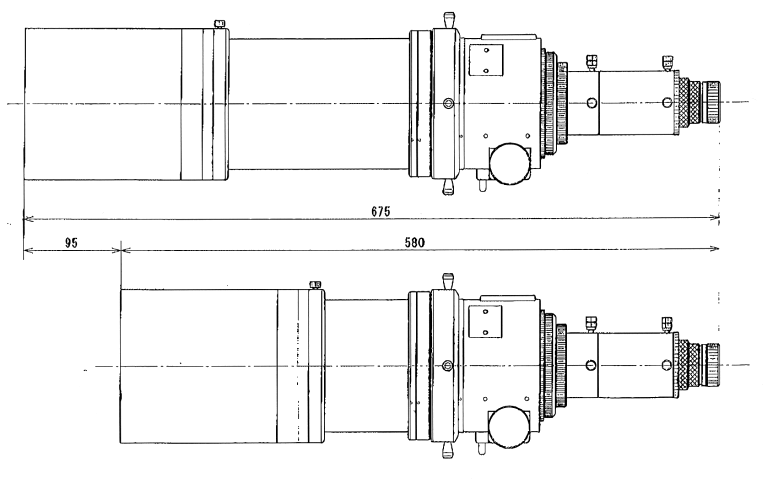
\includegraphics[width = 9cm]{FSQ_106ED_tube}
	\end{center}
	\caption{Takahashi사의 FSQ-106ED의 사양 \cite{fsq106ed}.}
	\label{FSQ}
\end{figure}


\subsection{구동부 제작}

\subsubsection{후드 제작}
Fusion360(https://www.autodesk.co.kr/products/fusion-360/students-teachers-educators)을 이용하여 \textrm{Figure} \ref{coverpeice}와 같이 경통의 후드를 설계한 후, 3D 프린터로 출력하여 후드를 제작하였다. 경통의 후드는 천체망원경 별로 경통의 지름과 같은 특성이 다르고, 천체망원경 위에 고정시킬 수 있을 만큼 견고해야한다. 때문에 경통에 씌울 수 있도록 지름을 계산하여 팔각형 모양으로 감싸는 형태로 제작하였으며, 3D 프린터에서 출력할 수 있는 크기 제한이 있고 동시에 천체망원경에 부착시킬 때 편리하게 할 수 있도록 총 네 조각으로 나누어 조립하는 방식을 택하였다. 네개 조각의 렌치 볼트와 너트로 조립하여 완성할 수 있다.

\begin{figure}[h]
	\begin{center}
		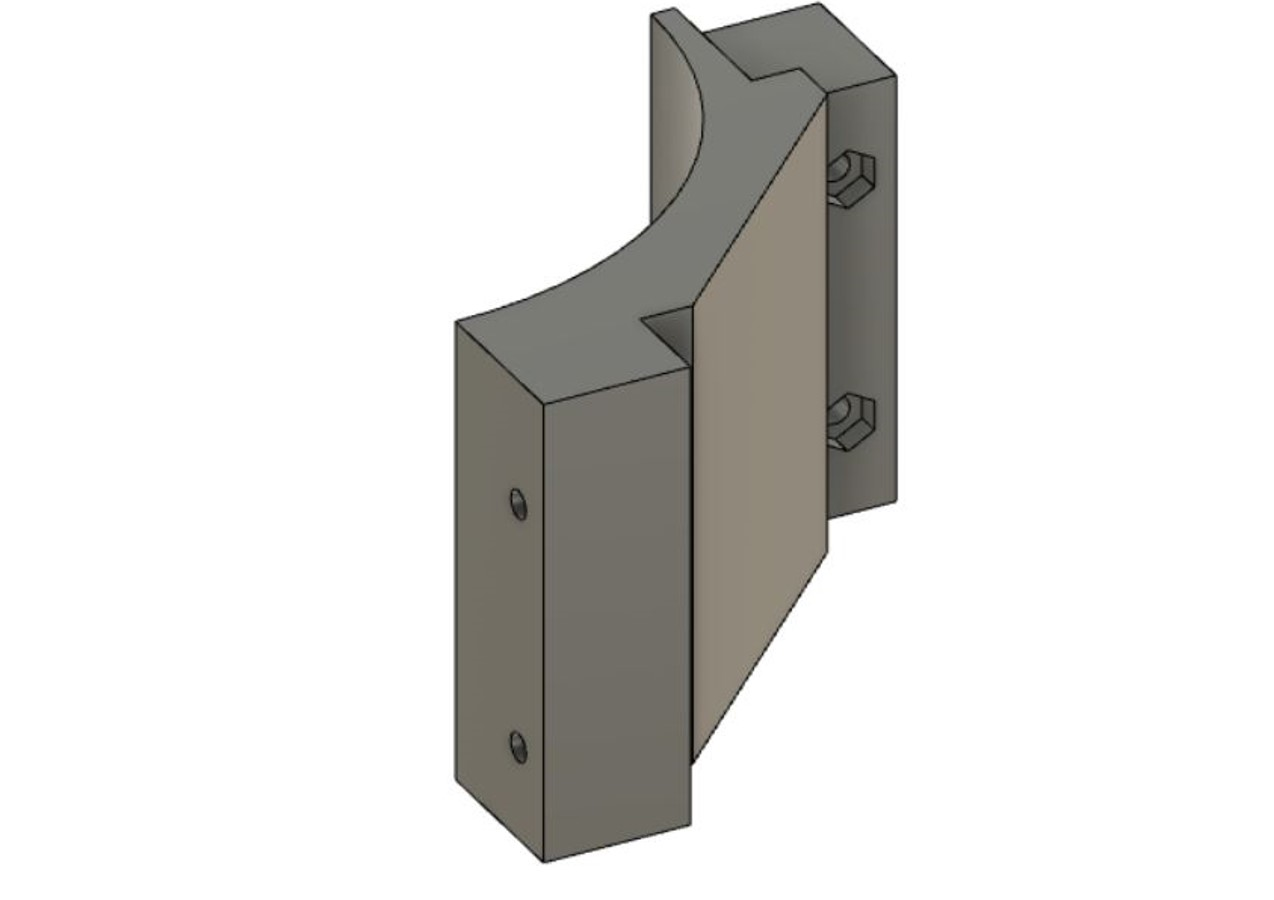
\includegraphics[width = 6.5cm]{coverpeice1}
		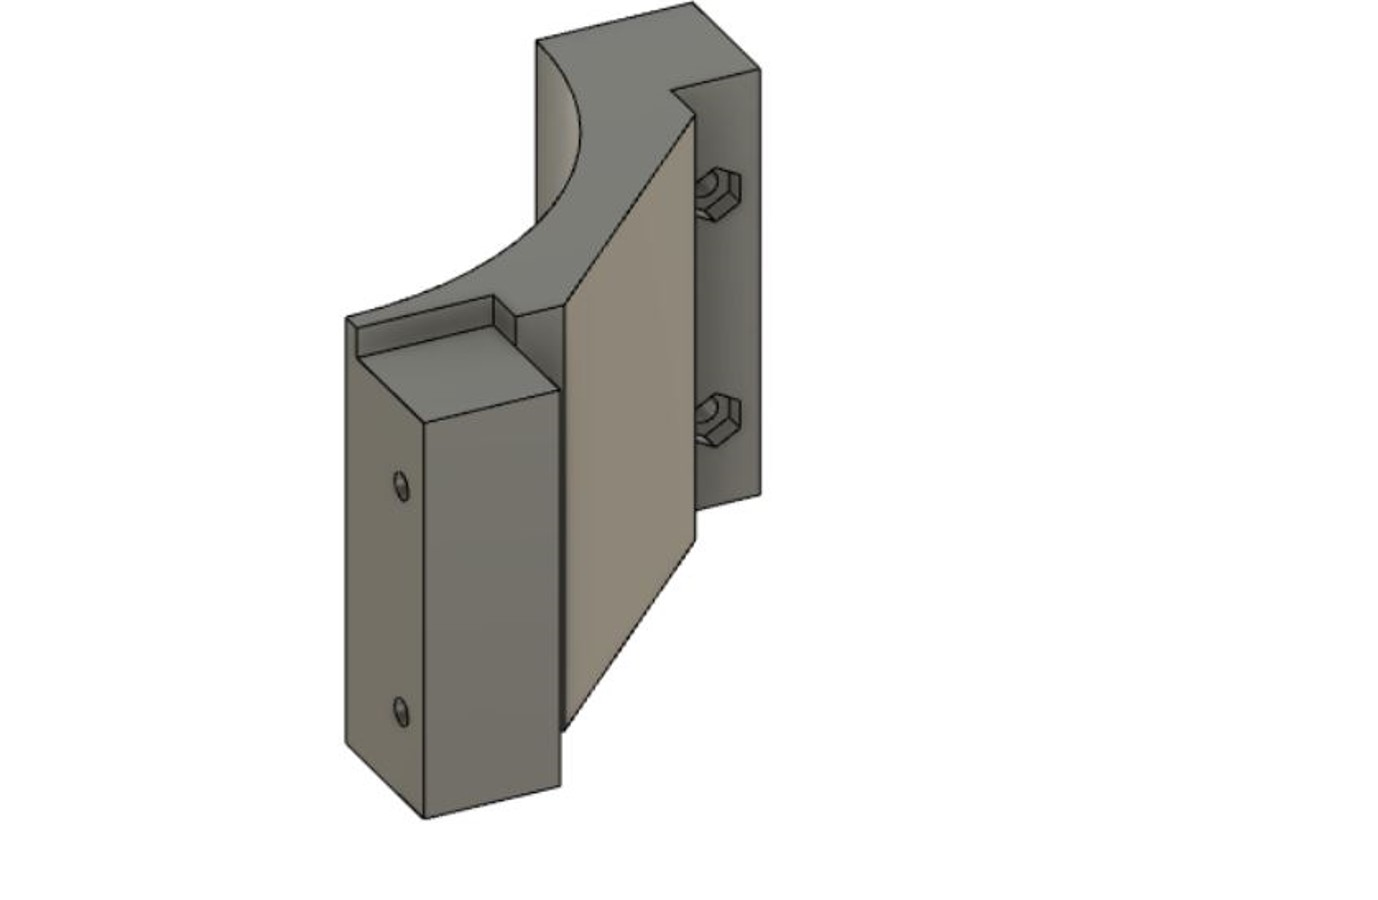
\includegraphics[width = 7.5cm]{coverpeice2}
	\end{center}
	\caption{Fusion360을 이용하여 설계한 경통 덮개 조각들}
	\label{coverpeice}
\end{figure}

본 연구에서는 부품들을 3D 프린터로 출력 후 조립하여 \textrm{Figure} \ref{cover}와 같이 이를 천체망원경의 후드처럼 부착시키는 것에 성공하였다. 후드의 지름은 망원경에 따라 달라질 수 있으므로 다른 망원경에 대한 후드를 제작할 때에는 이에 맞추어 새로 제작하여야 한다.

\begin{figure}[h]
	\begin{center}
		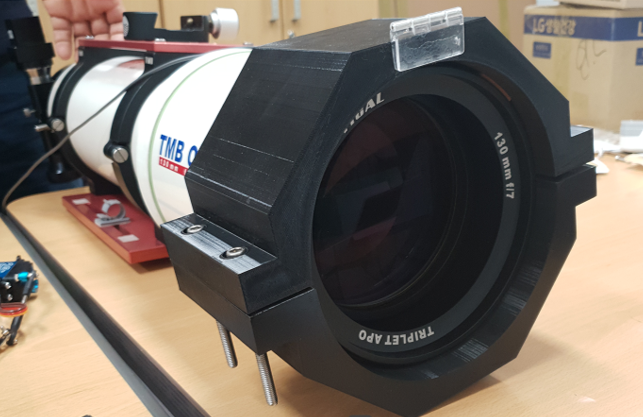
\includegraphics[width = 8cm]{cover}
	\end{center}
	\caption{제작한 후드를 천체망원경에 장착한 모습}
	\label{cover}
\end{figure}


\subsubsection{아크릴 덮개 제작}

천체망원경의 자동화를 실현하기 위해서는 경통의 덮개를 열고 닫는 것이 필요한데 소형 천체망원경의 경우 이러한 기능이 개발되어 있지 않다. 천체망원경의 광학계는 사용하지 않을 때에는 먼지, 이슬 등의 피해를 최소화 하기 위하여 덮개를 덮어 두어야 하고, 관측시에만 덮개를 열고 관측하는 것이 바람직하다. 

이에 제작한 후드에 꼭 맞는 크기로 아크릴을 가공하여 덮개를 제작한 경첩을 달아 서보모터로 열고 닫을 수 있도록 설계하였다. 처음에는 \textrm{Figure} \ref{cover}와 같이 아크릴 경첩을 이용하였으나 내구성에서 문제가 있다고 판단되어 견고하게 제작하기 위하여 금속 경첩으로 교체하였다. 금속으로 제작된 경첩은 볼트로 체결하는 방식으로 후드와 안정적으로 결합할 수 있었으며, 내구성 또한 뛰어났기 때문에 서보모터로 열고 닫느데 문제가 없었다. \textrm{Figure} \ref{hinge}와 같이 금속 재질의 경첩은 덮개와 아크릴 바흐티노프 마스크 사이를 납작볼트를 이용하여 연결할 수 있으며, 이는 접착제를 이용하여 붙이는 방법보다 간단하고 견고하게 조립되었다.

\begin{figure}[h]
	\begin{center}
		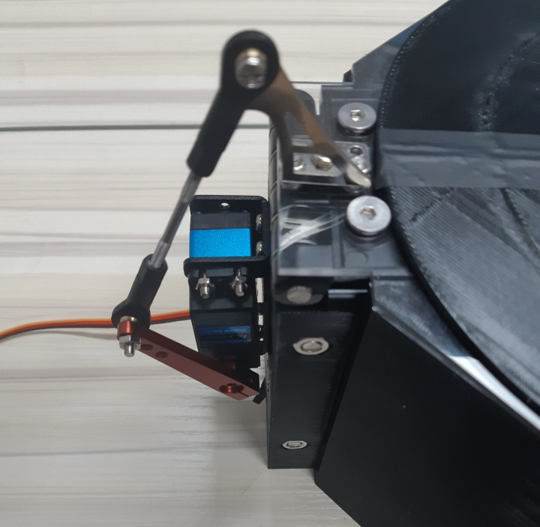
\includegraphics[width = 6cm]{hinge}
	\end{center}
	\caption{개선한 경첩 및 서보모터}
	\label{hinge}
\end{figure}

경통의 후드에서 바흐티노프마스크를 확실하게 제어하기 위해서는 바흐티노프마스크를 적용할 때와 적용하지 않을 때의 구분이 확실해야한다. 이를 확실하게 하기 위해서 바흐티노프마스크를 경첩을 이용하여 큰 각도로 제어하는 방법을 택하였으며, 이를 위해 덮개를 설계할 때 \textrm{Figure} \ref{coverpeice}와 같이 경첩의 높이를 고려하여 제작하였다.

서보모터는 일반적으로 사용하는 DC모터와 다르게 원하는 각도로 모터의 속도를 조절하여 이동시킬 수 있는 모터로,  RC카의 방향제어, 로봇의 관절제어 등의 상황에서 자주 사용되곤 한다. 본 연구에서 사용되는 서보모터는 ‘ds lx3325mg 25kg’ 모델(\textrm{Figure} \ref{motor})으로, 서보모터이지만 360도 회전이 가능한 모델으로, 몸체가 금속으로 되어있어 내구성을 기대할 수 있으며, 축이 톱니모양으로 되어 있기 때문에 제어가 편리하다는 장점을 가지고 있다.

\begin{figure}[h]
	\begin{center}
		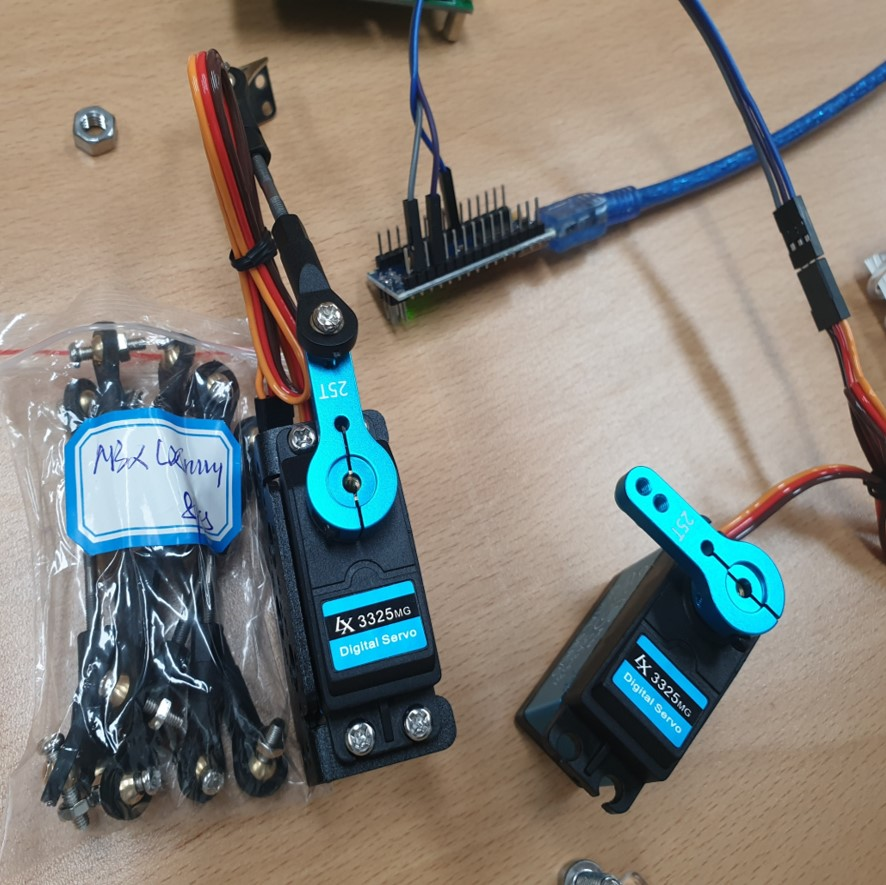
\includegraphics[width = 7cm]{servo1}
	\end{center}
	\caption{사용한 서보모터인 ds lx3325mg 25kg}
	\label{motor}
\end{figure}

\begin{figure}[h]
	\begin{center}
		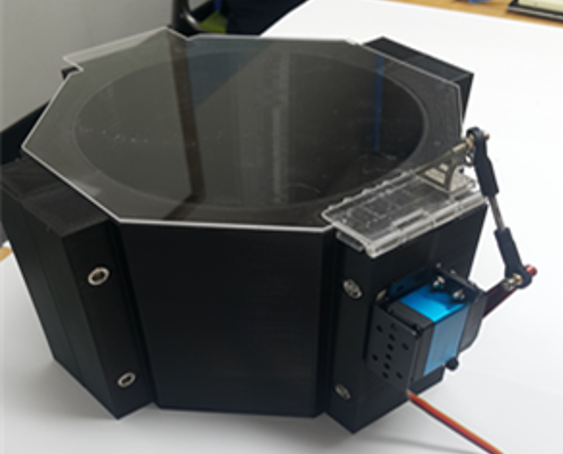
\includegraphics[width = 7.5cm]{servo2}
	\end{center}
	\caption{서보모터를 제작한 후드에 장착한 모습.}
	\label{motorcover}
\end{figure}

서보모터의 경우 구동을 위해 필요한 핀은 3가지이며, 일반적으로 주황색, 빨간색, 갈색의 핀으로 이루어져 있다. 주황색 핀은 모터를 제어할 수 있는 핀이며, 빨간색 핀과 갈색 핀은 각각 $\textrm{5 V}$ 전원과 GND에 연결하여 서보모터를 구동할 수 있다. 서보모터의 경우 \textrm{Figure} \ref{motorcover}처럼 후드의 옆면에 부착시켜 일정한 각도로 제어할 수 있게끔 설계하였다.

서보모터는 후드의 옆면에 부착시켜 제어시킨다. 이 때 정확한 위치에 부착시킬 수 있도록 일정한 간격을 두어 실험을 반복하였으며, \textrm{Figure} \ref{servo}와 같이 적합한 위치를 찾아 고정시켰다. 서보모터로 마스크를 정확하게 제어하기 위해서는 마스크가 완전히 덮개에 고정될 수 있어야 하므로 이에 맞는 각도를 계산하여 사용하여야 한다.

\begin{figure}[ht]
	\begin{center}
		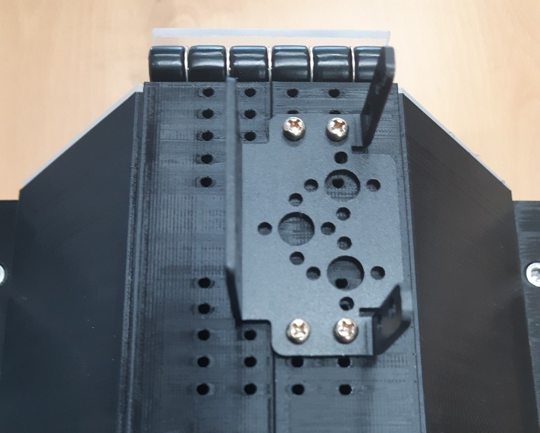
\includegraphics[width = 7cm]{servo3}
	\end{center}
	\caption{후드에 서보모터를 고정하기 위해 볼트를 이용해 고정한 모습}
	\label{servo}
\end{figure}


\subsubsection{바흐티노프마스크 제작}
천체망원경에 사용되는 대부분의 바흐티노프마스크의 도안은 직접 제작이 가능하며, 본 연구의 경우 astrojargon (http://astrojargon.net/MaskGenerator.aspx) 사이트에서 망원경의 사양 및 마스크의 사용 목적에 맞는 적절한 바흐티노프마스크의 도안을 제작하여 사용하였다.

덮개에서 사용되는 방식을 이용한 바흐티노프마스크의 경우 기존처럼 종이나 알루미늄에 프린트된 방식일 경우 덮개에 원하는 모양으로 씌워지지 않을 가능성이 있다. 때문에 주변환경에 영향을 적게 받으면서도 그 면이 평평하여 천체관측을 진행할 때에 영향이 없어야 한다. 

연구 초기에는 아크릴이 이러한 성질을 만족하면서도 쉽게 제작할 수 있으므로 아크릴에 레이저를 쐬여 바흐티노프마스크 모양을 씌우는 방법으로 테스트용 마스크를 제작해보았으나. 이러한 방식을 사용할 경우 \textrm{Figure} \ref{bendmask}처럼 레이저로 인해 열을 받은 아크릴이 변형되어 정밀한 초점 조절이 불가능해지는 경우가 발생하였으며, 아크릴의 두께로 인해 실제로 초점을 조절할 때에 걸리는 여러 가지 변수 또한 무시할 수 없었다.

\bigskip
\begin{figure}[h]
	\begin{center}
		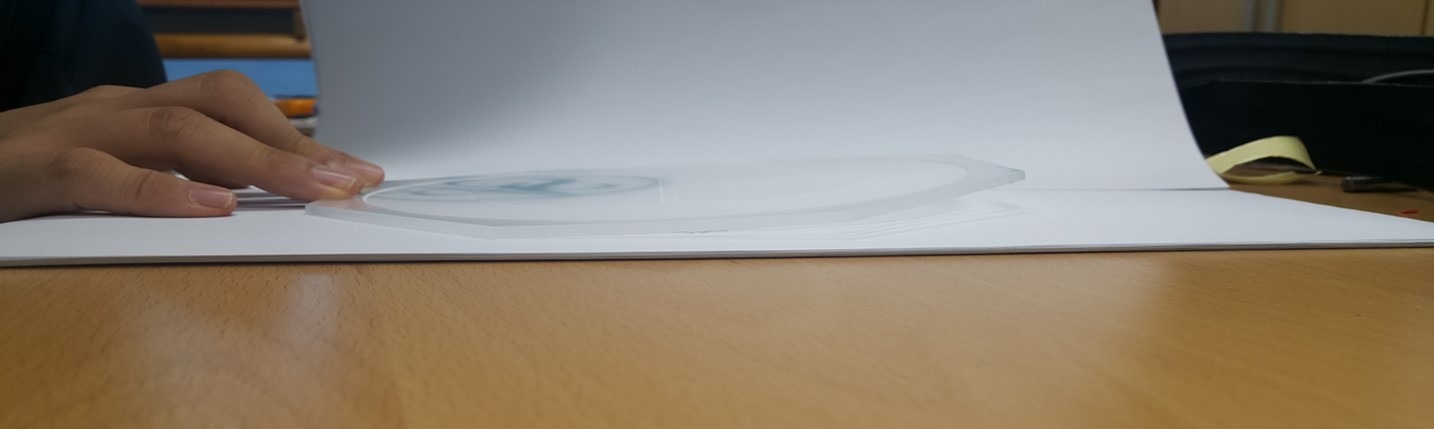
\includegraphics[width = 12 cm]{bendmask}
	\end{center}
	\caption{레이저에 의해 휘어진 아크릴 마스크}
	\label{bendmask}
\end{figure}

때문에 선택한 새로운 방법은 3d프린터를 이용하여 바흐티노프 마스크를 출력하는 것이다. 이 방법으로 얇으면서도 딱딱한 마스크를 사용할 수 있으므로 일반적인 아크릴을 활용한 마스크보다 적은 변수로 바흐티노프 마스크를 덮개에 부착시킬 수 있었다.

Astrojargon을 이용하여 출력한 바흐티노프마스크는 D값을 106, focal length 값을 530으로 출력하였으며, 덮개의 아크릴에 붙이기 편리하도록 지름을 아크릴과 같은 크기로 제작하였다. 출력 과정 중 바흐티노프 사이즈의 크기가 크기 때문에 4조각으로 나누어서 출력하였으며, 빛이 새는 것을 방지하기 위해 나중에 이를 검은 색 테이프로 봉합하였다. 

\begin{figure}[ht]
	\begin{center}
		\begin{tikzpicture}
		\node[anchor=south west,inner sep=0] at (0,0) 
		{
			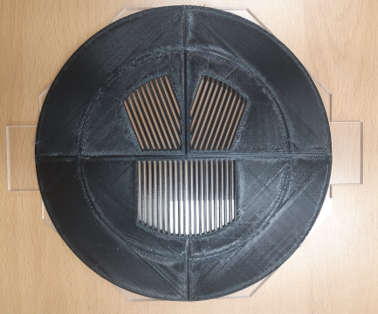
\includegraphics[height=4.5cm]{mask1}
			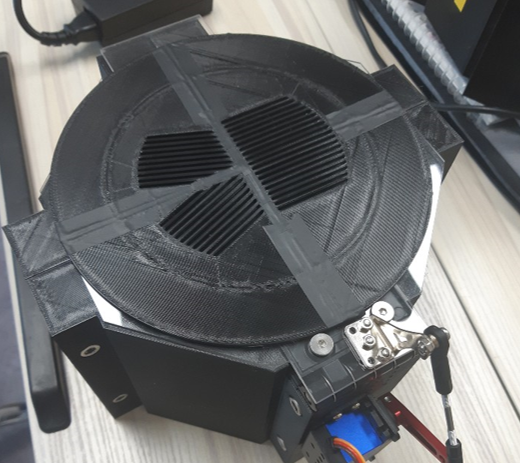
\includegraphics[height=4.5cm]{mask2} 
		};
		\draw (0.3, 4.2) node {(a)};
		\draw (5.9, 4.2) node {(b)};
		\end{tikzpicture}
	\end{center}
	\caption{(a) 4 조각으로 나누어서 출력한 FSQ-106ED 경통의 바흐티노프 마스크 (b) 출력된 마스크를 경통에 붙인 모습. 빛이 새지 않도록 접착부를 검은색 테이프로 접합시켜 고정하였다.}
	\label{mask}
\end{figure}

또한, 3D 프린터의 특성상 한쪽 면은 거친 면, 다른 한쪽 면은 평평한 면을 가지고 있는다. 이 때 거리를 일정하게 하기 위해 평평한 면이 아크릴과 붙는 방향으로 고정시켰다.

\subsubsection{열선 제작}
열선은  니크롬선을 이용하여 제작하였으며, 망원경의 크기와 필요한 열량 등을 고려하여 니크롬선의 저항을 선택한다.

\begin{figure}[h]
	\begin{center}
		\begin{tikzpicture}
		\node[anchor=south west,inner sep=0] at (0,0) 
		{
			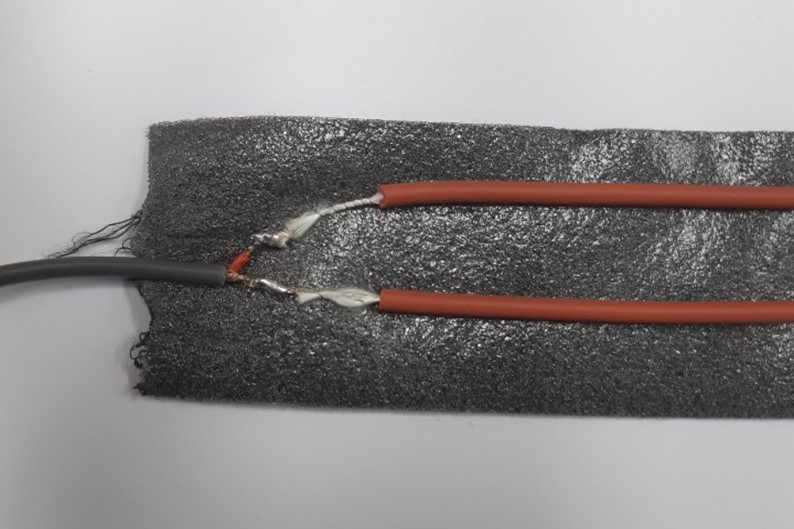
\includegraphics[width=6cm]{thermicline1}
			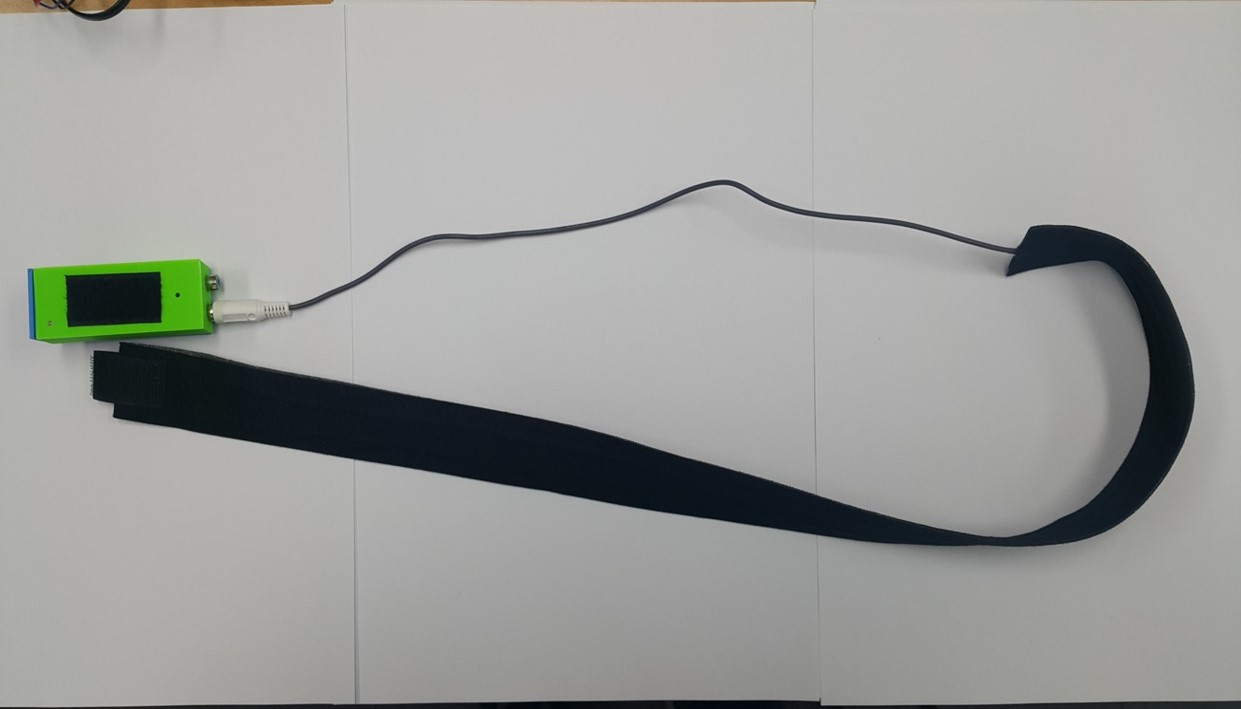
\includegraphics[width=7cm]{thermicline3} 
		};
		\draw (0.3, 3.7) node {(a)};
		\draw (6.4, 3.7) node {(b)};
		\end{tikzpicture}
	\end{center}
	\caption{(a) 제작한 열선의 접합부와 (b) 제작한 열선을 12V에 연결한 모습. 끝에 벨크로가 붙어있어 경통에 둘러 사용할 때 편리하다.}
	\label{thermic}
\end{figure}

열선을 제작하는 방법은 간단하다. 먼저 \textrm{Figure} \ref{thermic}a처럼 끈끈한 면에 히팅케이블을 부착한 뒤에 알맞는 12V어댑터를 분해하여 극을 선과 연결한다. 그리고 열선을 다시 덮어주게 되면 12V 전원을 통해 작동하는 열선을 제작할 수 있다. 열선을 실제로 사용할 시에는 그 편의성을 증대시키기 위해 열선의 끝부분을 벨크로로 연결할 수 있도록 만들게 되며, 이렇게 제작한 열선은 렌즈가 있는 부분을 찾아 둘러주면 벨크로로 끝을 고정시켜 쉽게 망원경에 부착시킬 수 있다.


\subsection{제어부 제작}

\subsubsection{회로 구성}

\textrm{Figure} \ref{circuit01}와

\begin{figure}[h]
	\begin{center}
		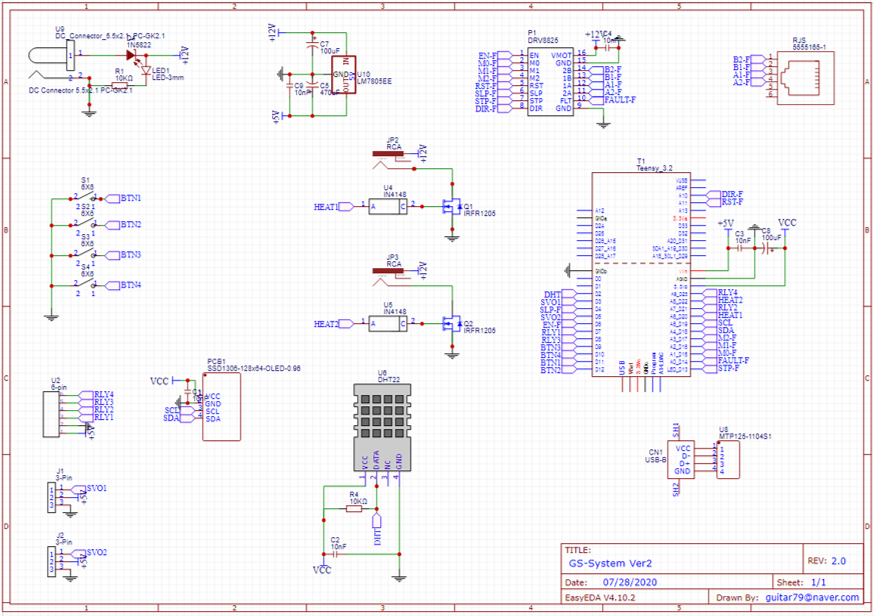
\includegraphics[width = 12cm]{circuit01}
	\end{center}
	\caption{제어부 회로도}
	\label{circuit01}
\end{figure}



\subsubsection{전원 제어}

릴레이 스위치는 전자석으로 이루어진 여러 스위치를 한번에 제어할 수 있도록 제작된 장비이다. 천체관측을 시작 및 종료할 때 가대, CCD, 카메라 등 한번에 여러 가지의 전원을 제어해야 하는데, 릴레이 스위치를 이용하면 한번에 제어할 수 있어 편리하다. 

\begin{figure}[h]
	\begin{center}
		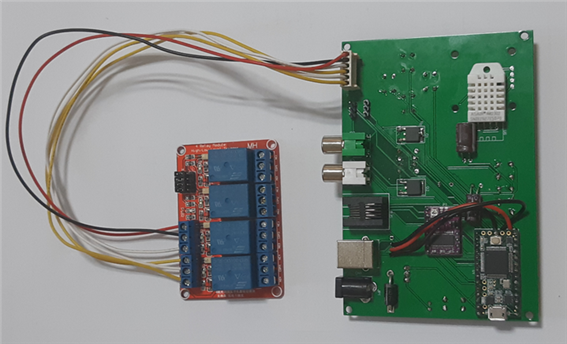
\includegraphics[width = 7.5cm]{relay}
	\end{center}
	\caption{실험에 사용된 릴레이스위치를 모터포커서에 연결시킨 모습}
	\label{relay}
\end{figure}


\textrm{Figure} \ref{relay}와 같이 각각의 스위치를 선으로 연결시켜 mcu의 각 핀에 연결시켜 작동시킬 수 있으며, 함수로 지정하여 이들을 한번에 제어할 수 있도록 하였다.

릴레이 스위치는 6개의 핀으로 이루어져 있으며, 순서대로 $\textrm{+5 V}$, GND, 1, 2, 3, 4의 Relay이다. 때문에 각 핀들을 모두 연결시킨 뒤에 MCU를 이용하여 적절하게 제어할 수 있다. 각각의 기호는 P, Q, R, S이며, 상태만을 나타내기 때문에 서보모터 제어와 마찬가지로 오직 0과 1만을 입력받는다.



\subsubsection{모터 포커서 제어}

이전에 개발된 GS-touch는 바이폴라 스테핑 모터를 제어할 수 있는 모터 포커서로 초점 조절 기능은 이기 때문에 이를 위한 기능들이 주를 이루었다. 때문에 이를 보완하여 덮개를 제어할 수 있도록 추가로 개발할 필요가 있다.


\textrm{Figure} \ref{GStocuh}는 기존에 사용하는 GS-touch의 주요 기능들을 정리한 표이며, GS-touch는 전체적으로 두 가지 부분으로 나눌 수 있다.

\bigskip
\begin{figure}[h]
	\begin{center}
		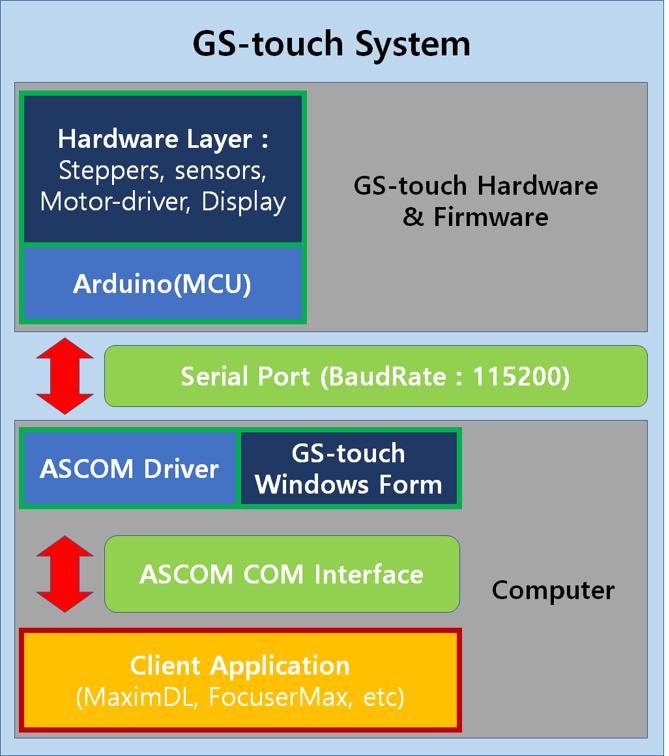
\includegraphics[width = 9.7cm]{GStouch}
	\end{center}
	\caption{GS-touch의 주요 기능}
	\label{GStocuh}
\end{figure}

첫 번째로 GS-touch의 펌웨어는 모터를 직접적으로 제어할 수 있다. DRV8825 모터 드라이버를 활용하여 최대 1/32step의 마이크로 컨트롤을 지원하기 때문에 정밀하게 경통의 길이를 조절할 수 있도록 설계되었으며, 이들을 편하게 관리할 수 있도록 움직인 만큼의 step을 디스플레이에 나타내주며, 이를 원하는 숫자로 초기화하여 얼마나 더 움직였는지 또한 알기 쉽게 하였다. 부가적인 기능으로는 현재 컨트롤러의 위치의 온도와 습도를 알 수 있도록 하여 주변 상황을 쉽게 알 수 있도록 하였다.

두 번째 부분은 GS-touch의 직접적인 제어가 가능하도록 하는 ASCOM 호환 드라이버이다. GS-touch의 드라이버는 ASCOM 홈페이지에서 제공하는 개발자용 버전을 응용하여 C\# 기반으로 제작되었으며, GUI 및 애플리케이션 소프트웨어를 제공하기 때문에 펌웨어에서 제공하는 모든 기능들을 컴퓨터에서 원격으로 사용할 수 있도록 하였다.


비록 GS-touch는 여러 가지 기능을 가지고 있지만 천체망원경의 원격조작에 필요한 여러 기능들을 완벽하게 갖추지는 못하였다. 대표적으로, EEPROM을 사용하지 않았기 때문에 원하는 길이에 step값을 저장할 수 없으며, 온도 및 습도 측정 외의 편의기능 또한 없기 때문에 실제로 사용할 때 많은 불편함이 있다. 본 연구에서는 이러한 단점들을 보완하여 EEPROM을 적용시키고 열선을 사용가능하도록 하는 등의 여러 편의기능들을 개선하였으며, 이를 사용하여 천체망원경용 덮개를 제어할 수 있도록 하였다. 앞으로 실제 천체관측에서의 활용성은 기존에 없었던 천체망원경용 덮개와 더불어 천체망원경의 원격 조작에 큰 도움을 줄 수 있을 것이다.


\subsubsection{서보모터 제어}
바흐티노프마스크를 제어하기 위해서 필요한 조건을 여러 가지가 있겠지만, 가장 중요한 조건 중 하나는 마스크를 사용하는 때와 그렇지 않을 때를 정확히 구분해야하며, 특히 마스크를 사용할 때에는 모든 상황에서 같은 환경을 제공할 수 있어야 한다. 본 연구에서는 경첩을 이용한 각도의 차이로 마스크를 제어하기 때문에 정확한 각도의 이동이 가장 중요하기 때문에 원하는 각도로 정확히 이동할 수 있는 서보모터를 사용하여 정확한 제어가 가능하도록 하였다.

%\subsection{기존 모터포커서 보강}

%앞서 소개했듯이 기존의 모터포커서인 GS-touch는 모터의 초점을 맞추기 위한 기능들에 집중이 되어있기 때문에, 실제로 천체관측 및 원격 천체관측에서는 사용하기 아쉬운 부분들이 많았다. 이에 기존 모터포커서를 보강하였으며, 기존 모터포커서에 비해서 원격 천체관측에 필요한 여러 가지 기능들을 탑재하였다. 본 연구에서 새로 보강한 부분은 다음과 같다.

\subsubsection{열선 제어}
열선또한 정확한 천체관측에 필요한 장비 중 하나이다. 관측을 진행할 때에 경통의 온도가 내려가면 렌즈에 이슬이 맺히게 되는데, 이는 정확한 상을 맺히게 하는데 크게 어려움을 주게 된다. 열선을 경통에 감아놓으면 경통의 온도에 따라서 열선을 제어하여 깨끗한 렌즈를 사용할 수 있게되므로 관측을 편리하게 할 수 있으며, 때문에 천체망원경을 원격제어하기 위해서는 온도를 측정할 수 있는 장비와 열선이 필수적이다. 

열선은 PWM(Puls Width Modulation)을 이용하여 세기를 조절할 수 있다. PWM은 디지털 신호의 밀도로 그 세기를 조절하는 방식으로다 디지털 신호인 0과 1이 출력되는 시간의 비율을 조절하여 원하는 밀도로 제어할 수 있도록 한다. 본 연구에서 직접 제작한 열선을 포함한 대부분의 열선은 12V의 전압을 이용해 제어해야하기 때문에 아두이노의 출력 전원인 5V로는 신호만 제어하고 스위칭 트랜지스터를 이용하여 12V의 전압을 PWM으로 제어할 수 있도록 설계하였다.


앞서 설명하였듯 열선의 제어는 전압의 PWM을 이용하여 실행된다. \textrm{Figure} \ref{PWM}와 같이 시리얼 포트를 통한 입력을 할 때 필요한 기호는 A와 D이며, 0~100의 값을 입력받아 500ms 주기로 값을 변화시킬 수 있도록 설계하였다.

\begin{figure}[ht]
	\begin{center}
		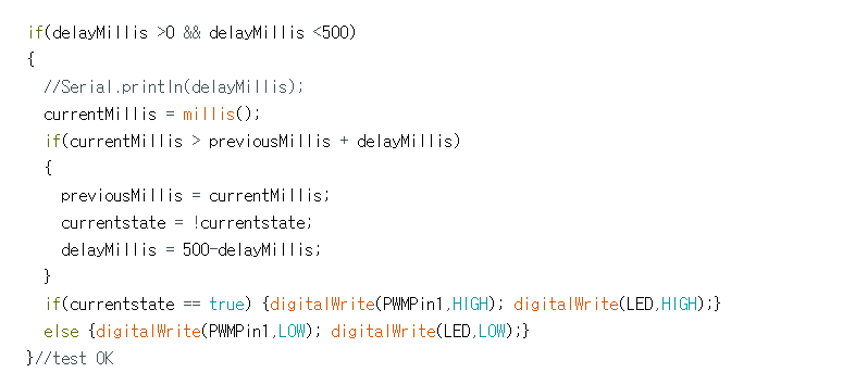
\includegraphics[width = 11cm]{PWMcode}
	\end{center}
	\caption{PWM제어를 위한 코드}
	\label{PWM}
\end{figure}

\subsubsection{EEPROM(Electrically Erasable Read-Only Memory)}

MCU(Micro Controller Unit)내에 원하는 값을 저장하는 방법은 여러 가지가 있다. 일반적으로 펌웨어가 실행되기 전에 변수를 선언하고, loop 문 속에 들어있는 여러 함수들을 통해 그 값을 바꾸는 방법을 사용하곤 한다. 하지만 원격 천체관측을 위한 펌웨어인 만큼, MCU내의 변수만으로 값을 저장하는 것은 상당히 위험하며, 그 전원을 계속 유지할 수 없기 때문에 다른 방법으로 값을 저장할 필요성을 느꼈으며, EEPROM은 기존 방법에 비해 안전하게 값을 저장할 수 있기 때문에 사용하게 되었다.

EEPROM은 대표적인 롬(ROM - read only memory)의 한 종류로서, 전원을 차단해도 저장된 정보를 유지하는 비휘발성 메모리이다. EEPROM은 address를 가지고 있어서 각각의 address 안에 지정된 bytes의 값을 저장할 수 있다. 본 연구에서 사용된 MCU인 Teensy 3.2는 0에서 1023까지의 address지를 가지고 있고 하나의 address에 2048byte, 즉 0부터 255까지의 수를 저장할 수 있다. 모터포커서의 step을 저장하기 위해서는 약 100000범위의 수를 저장할 필요가 있다. GS-touch는 약 -50000에서 50000까지의 수를 저장할 수 있기 때문에 256진법을 활용하여 수를 저장할 수 있도록 설계하였다.

\begin{figure}[h]
	\begin{center}
		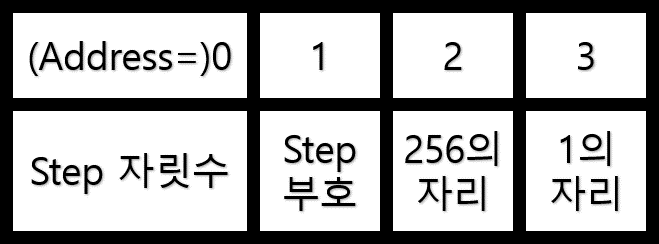
\includegraphics[width = 5 cm]{eeprom1}
	\end{center}
	\caption{EEPROM의 address별 사용 구조. 부호와 값을 절대치를 이용하여 연산하였다.}
	\label{eeprom1}
\end{figure}

\begin{figure}[ht]
	\begin{center}
		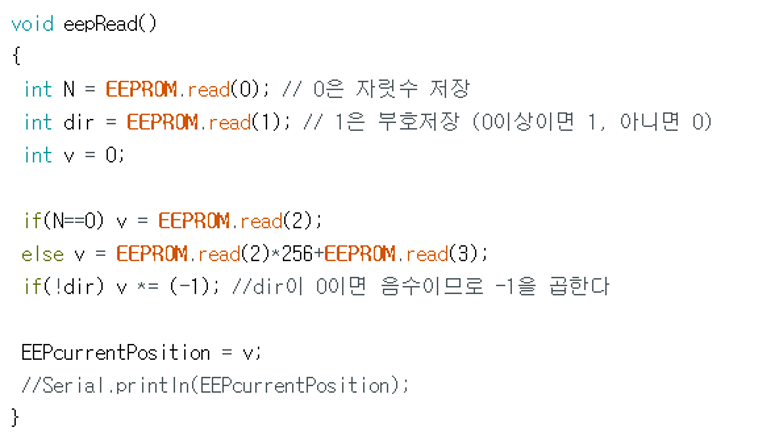
\includegraphics[width = 11cm]{eepread}
	\end{center}
	\caption{EEPROM에서 정보를 읽어오는 과정}
	\label{eepread}
\end{figure}

%https://www.pjrc.com/teensy/td_libs_EEPROM.html

 와 같이 작성
	%%%% 주의
	%%%% 파일이 나뉠 때마다 자동으로 페이지넘김(\clearpage)가 됩니다. 
	%%%% 따라서 subsection을 나누는 용도로는 사용하지 마십시오.
	%%%% \include{sub/experiment} 와 같이...
	
	\section{서론}

\subsection{연구의 필요성}

최근에는 천체 망원경이 대중화 되어 관측을 즐기는 인구가 많아 졌으며, 개인이 천체 망원경을 소유하여 장시간 노출을 필요로 하는 천체 사진 촬영을 즐기는 아마추어 천문인들도 온라인과 오프라인 동호회를 중심으로 많아지고 있다. Figure \ref{fig:The_Andromeda_Galaxy}\은 아마추어 천문가가 소형 천체망원경을 촬영한 안드로메다 은하의 사진이다. 이런 천체 사진을 촬영하기 위해서는 많은 노력이 필요하다.
\begin{figure}[h]
	\begin{center}
		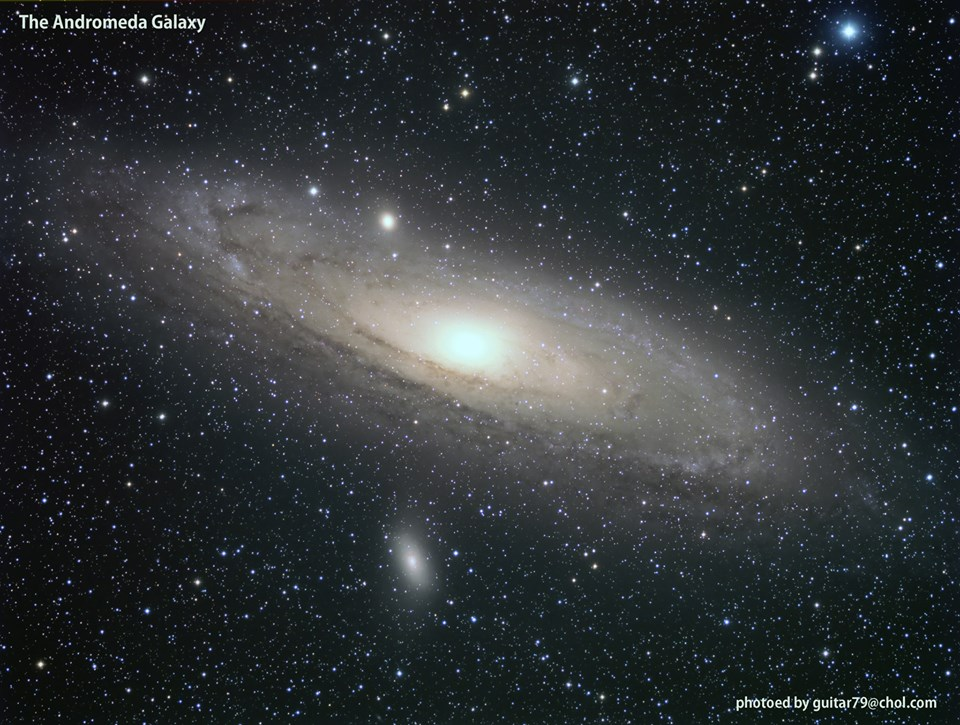
\includegraphics[width=0.95\linewidth]{Andromeda_Galaxy}
		\caption{The Andromeda Galaxy (Takahashi FSQ106-ED with 0.73X Reducer QE, Sbig ST-8300M, Takahashi EM-200 Temma 2) : L 600s X 14 frames, RGB 400s X 6 frames each.}
		\label{fig:The_Andromeda_Galaxy}
	\end{center}
\end{figure}

Figure \ref{fig:observing_system}\은 사진 관측을 하기 위한 천체 망원경 시스템을 보여 준다. 사진 관측을 위한 천체 망원경 시스템은 크게 광학계(optic), 검출기(detector), 마운트(mount)로 이루어지며, 정밀도를 높이기 위해 가이드 시스템을 포함한 여러가지 보조 도구들이 필요하다. 광학계의 결상 성능, 마운트의 추적 성능 등을 갖추고 있어야 오랜 시간동안 노출을 주며 천체 사진을 찍을 수 있게 된다. Figure \ref{fig:The_Andromeda_Galaxy}\은 Sbig(Santa Barbara Instrument Group)사의  ST-8300M이라는 모노크롬 CCD(Charge-coupled device)를 이용하여 촬영하였으며, 노출 정보를 보면 L(Luminence) 채널의 경우 600 sec의 노출로 14 frame을 촬영하여 합성하였으며, R(Red), G(Green), B(Blue) 각각의 채널에서 400 sec의 노출로 6 frame씩 촬영하여 합성한 것이다. 이처럼 고품질의 천체사진 한 장을 촬영하기 위해서 많은 노력이 필요하다. 

\begin{figure}[h]
\begin{center}
	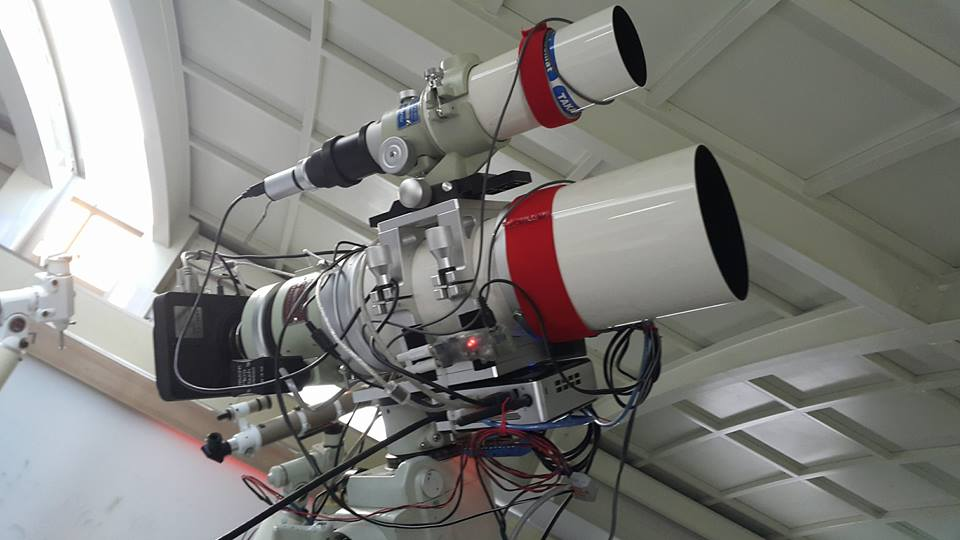
\includegraphics[width=0.8\linewidth]{observing_system}
	\caption{Telescope system for astrophotography}
	\label{fig:observing_system}
\end{center}
\end{figure}

광학계에 의한 별의 상이 검출기에 정확하게 맺히도록 하기 위해서는 포커서를 정밀하게 움직여야 한다. 사진 촬영을 위한 고성능의 광학계는 포커서(Focuser)를 견고하게 만들 뿐 아니라 포커서 노브에 미동 장치가 있어 정밀하게 초점 조절이 가능하다. 하지만 포커서를 조절하기 위해 손을 가져다 대기만 해도 그 진동이 상에 영향을 미치기 때문에 손으로 초점을 조절하는 

사천체를 관측할 때 초점을 맞춘다면 관측할 천체의 모습이 더 선명하게 보인다. 일반적으로 대부분 망원경은 초점을 손으로 맞출 수 있게 설계되어있다. 천체망원경으로 사진 관측을 할 때 정확한 초점 조절은 사진의 품질에 영향을 미치는 요소 중의 하나이다. 초점 조정 시 어려운 점은 초점을 조정하기 위해 초점 조절 노브에 손이 닿으면 진동이 발생하고, 그 진동이 사진의 품질에 영향을 준다. 또한, 초점을 조절할 때 손으로 돌리는 것은 미세한 조정에는 어려움이 있다. 또한, 초점이 완벽하게 맞지 않았는데도 이러한 사진을 찍기 위해서 초점을 맞추는데 많은 시간을 투자해야 한다. 이렇듯 사진을 통하여 정밀한 천체의 사진이 필요한 경우 사람의 손으로는 무리가 있다. 하지만 모터 초점 조절 장치가 있다면 손으로 초점을 맞추는 것보다 정확하게 초점을 맞출 수 있게 된다. 

The present invention provides a temperature compensating focuser and method for use with a telescope having a focus which changes with ambient temperature. \cite{persha2001temperature}
\begin{figure}[h]
	\begin{subfigure}{0.5\textwidth}
		
\includegraphics[width=0.9\linewidth, height=5cm]{before} 
		\caption{초점 맞추기 전}
		\label{fig:before}
	\end{subfigure}
	\begin{subfigure}{0.5\textwidth}
		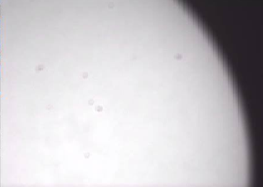
\includegraphics[width=0.9\linewidth, height=5cm]{after}
		\caption{초점 맞춘 후}
		\label{fig:after}
	\end{subfigure}
	\caption{초점을 맞추기 전과 후 비교}
	\label{fig:image1}
\end{figure}






Fig.1.(a), Fig.1.(b)에서 알 수 있듯이 모터 초점 조절 장치를 이용하여 초점을 맞추면 아무것도 하지 않고 그냥 관측했을 때에 비해서 훨씬 정확하게 천체를 관측할 수 있게 된다. Fig.1.(a)와 Fig.1.(b)를 비교하여 보면 Fig.1.(b)의 표면이 훨씬 더 선명하다는 사실을 알 수 있다. 하지만, 모터를 이용하여 초점을 맞춘다고 해도 우리 눈으로 초점을 맞추는 것이기 때문에 정확하지 않을 수 있다. 이러한 문제를 해결하기 위하여 만들어진 자동 초점 조절 장치가 있다. 자동 초점 조절 장치가 현재 개발된 제품이 미국 Starizona 회사의 Micro Touch이다. 이 제품은 자동 초점 조절 시스템이 구현이 잘 되어 있으나, 가격이 499달러로 부담 이 있을 수 있다. 또한, 실제로 모터 초점 조절 장치와 연계해 초점을 맞춰주는 다른 Software도 몇 종류가 있으나 오류가 발생하는 경우가 있다. 따라서 천체망원경의 모터 초점 조절 장치의 컨트롤러 구동 시스템을 개발하면 여러 천체를 관측하는 데 있어서 보다 정확한 사진들을 얻을 수 있을 것이다.

%\begin{wrapfigure}{l}{0.3\textwidth}
%	
\includegraphics[width=1\linewidth]{before}
%	\caption{초점 맞추기 전}
%	\label{fig:before}
%\end{wrapfigure}

\subsection{연구 목적}

본 논문에서 제안된 방법은 사람이 손으로 제어하는 것보다 정밀하고 빠르게 천체망원경의 초점을 맞출 수 있도록 편의성을 제공하기 위한 기반을 제공하기 위함이다. 이 연구는 Arduino를 이용하여 천체망원경을 이용한 천체관측을 시행할 때 필요한 모터 초점 조절 장치를 조정할 수 있는 모터 초점 조절 장치 컨트롤러 구동 시스템을 구현하고, 초점을 조정하는 알고리즘을 만들어서 천체의 초점을 맞출 수 있도록 한다. 그리고 이와 통신을 할 수 있는 시스템도 개발하여 편의성을 늘리고, ASCOM 드라이버를 제작하여 컴퓨터와의 통신을 가능하게 하는 것이 이 연구의 목표이다.
 % Introduction
	%\section{이론적 배경}

\section{연구 과정 및 방법}


\subsection{소형 천체망원경 자동화 시스템 구성}



%본 연구에서 사용되는 망원경은 기존 천체관측에 있어서 큰 어려움은 없어 원격 천체관측을 진행할 수 있어야 하며, 직접 덮개를 개발하게 되므로 적절한 크기를 가지고 있어야 한다. 최종적으로 선발된 망원경은 Takahashi 사의 'FSQ-106ED'이다. Takahashi 사의 웹사이트에서 참고한 FSQ-106ED의 스펙은 \textrm{Figure} \ref{FSQ}를 참고할 때 망원경의 경통은 580mm/675mm의 길이를 가지고 있으며, 지름은 125mm으로 마스크를 위한 덮개를 제작할 적절한 크기를 가지고 있다.

\begin{figure}[h]
	\begin{center}
		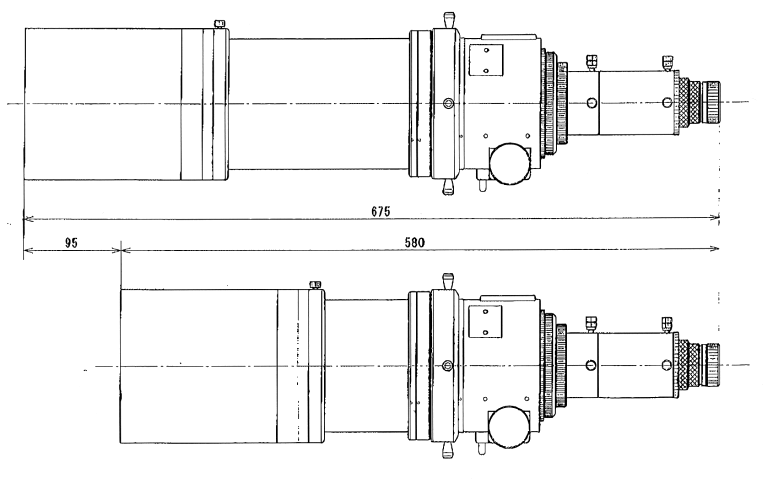
\includegraphics[width = 9cm]{FSQ_106ED_tube}
	\end{center}
	\caption{Takahashi사의 FSQ-106ED의 사양 \cite{fsq106ed}.}
	\label{FSQ}
\end{figure}


\subsection{구동부 제작}

\subsubsection{후드 제작}
Fusion360(https://www.autodesk.co.kr/products/fusion-360/students-teachers-educators)을 이용하여 \textrm{Figure} \ref{coverpeice}와 같이 경통의 후드를 설계한 후, 3D 프린터로 출력하여 후드를 제작하였다. 경통의 후드는 천체망원경 별로 경통의 지름과 같은 특성이 다르고, 천체망원경 위에 고정시킬 수 있을 만큼 견고해야한다. 때문에 경통에 씌울 수 있도록 지름을 계산하여 팔각형 모양으로 감싸는 형태로 제작하였으며, 3D 프린터에서 출력할 수 있는 크기 제한이 있고 동시에 천체망원경에 부착시킬 때 편리하게 할 수 있도록 총 네 조각으로 나누어 조립하는 방식을 택하였다. 네개 조각의 렌치 볼트와 너트로 조립하여 완성할 수 있다.

\begin{figure}[h]
	\begin{center}
		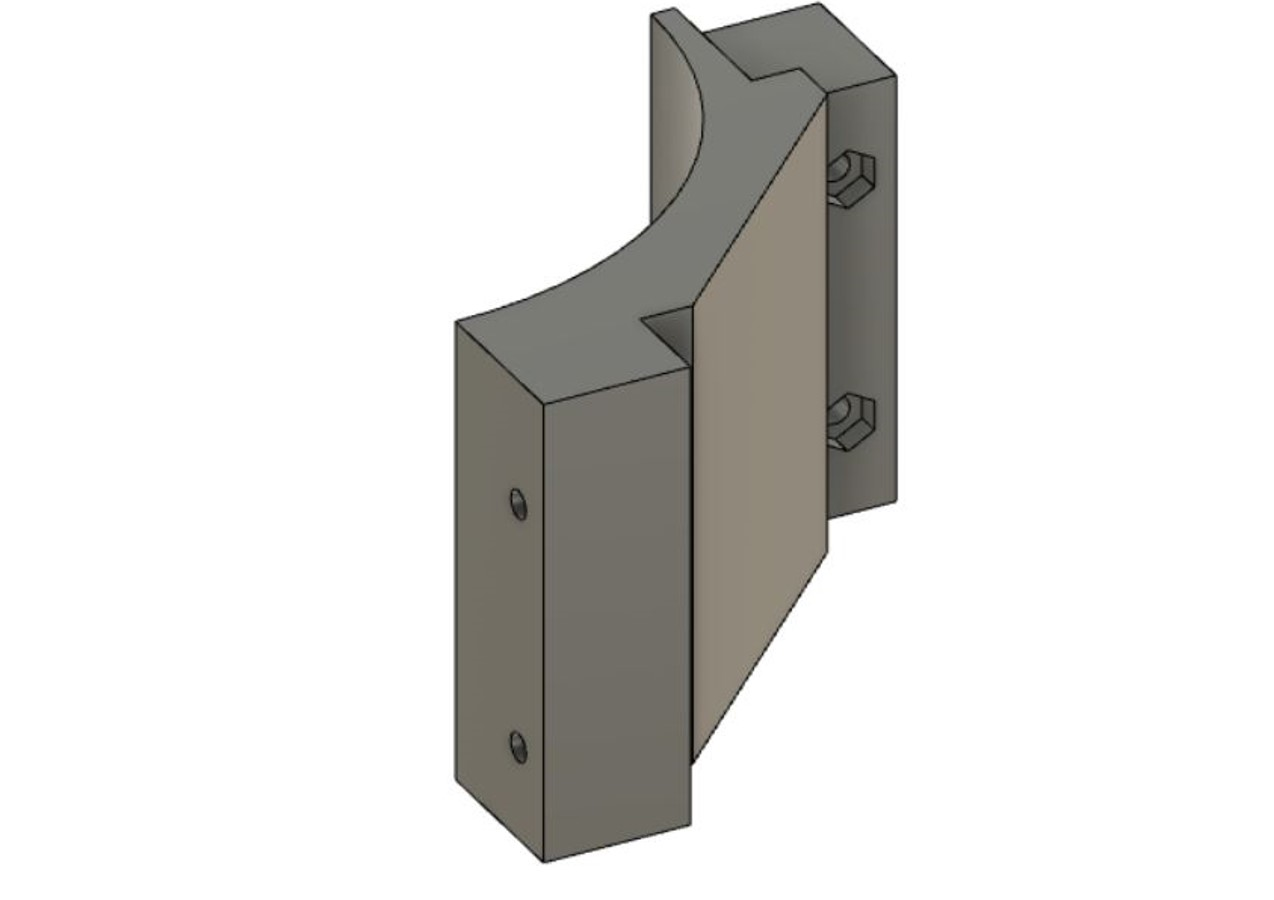
\includegraphics[width = 6.5cm]{coverpeice1}
		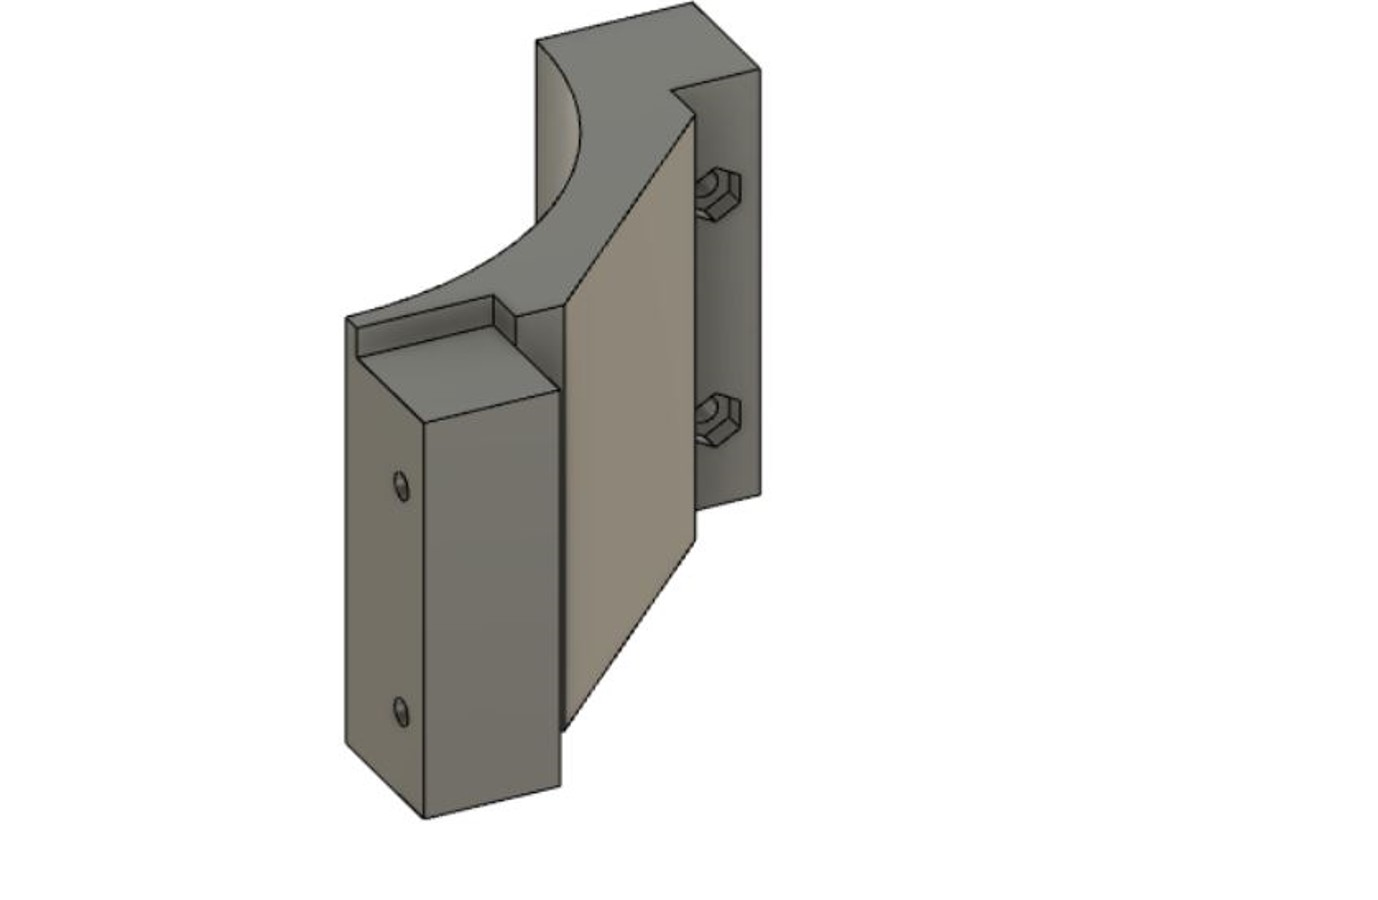
\includegraphics[width = 7.5cm]{coverpeice2}
	\end{center}
	\caption{Fusion360을 이용하여 설계한 경통 덮개 조각들}
	\label{coverpeice}
\end{figure}

본 연구에서는 부품들을 3D 프린터로 출력 후 조립하여 \textrm{Figure} \ref{cover}와 같이 이를 천체망원경의 후드처럼 부착시키는 것에 성공하였다. 후드의 지름은 망원경에 따라 달라질 수 있으므로 다른 망원경에 대한 후드를 제작할 때에는 이에 맞추어 새로 제작하여야 한다.

\begin{figure}[h]
	\begin{center}
		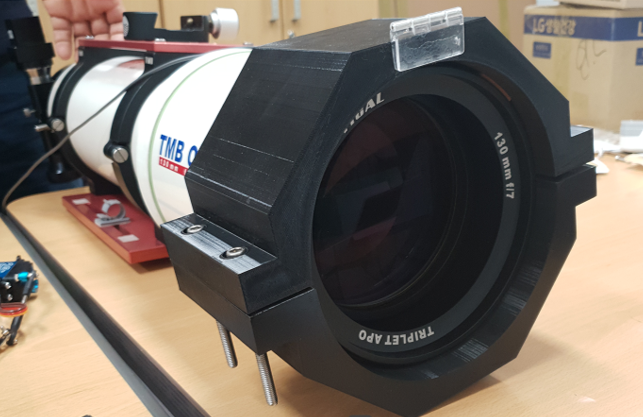
\includegraphics[width = 8cm]{cover}
	\end{center}
	\caption{제작한 후드를 천체망원경에 장착한 모습}
	\label{cover}
\end{figure}


\subsubsection{아크릴 덮개 제작}

천체망원경의 자동화를 실현하기 위해서는 경통의 덮개를 열고 닫는 것이 필요한데 소형 천체망원경의 경우 이러한 기능이 개발되어 있지 않다. 천체망원경의 광학계는 사용하지 않을 때에는 먼지, 이슬 등의 피해를 최소화 하기 위하여 덮개를 덮어 두어야 하고, 관측시에만 덮개를 열고 관측하는 것이 바람직하다. 

이에 제작한 후드에 꼭 맞는 크기로 아크릴을 가공하여 덮개를 제작한 경첩을 달아 서보모터로 열고 닫을 수 있도록 설계하였다. 처음에는 \textrm{Figure} \ref{cover}와 같이 아크릴 경첩을 이용하였으나 내구성에서 문제가 있다고 판단되어 견고하게 제작하기 위하여 금속 경첩으로 교체하였다. 금속으로 제작된 경첩은 볼트로 체결하는 방식으로 후드와 안정적으로 결합할 수 있었으며, 내구성 또한 뛰어났기 때문에 서보모터로 열고 닫느데 문제가 없었다. \textrm{Figure} \ref{hinge}와 같이 금속 재질의 경첩은 덮개와 아크릴 바흐티노프 마스크 사이를 납작볼트를 이용하여 연결할 수 있으며, 이는 접착제를 이용하여 붙이는 방법보다 간단하고 견고하게 조립되었다.

\begin{figure}[h]
	\begin{center}
		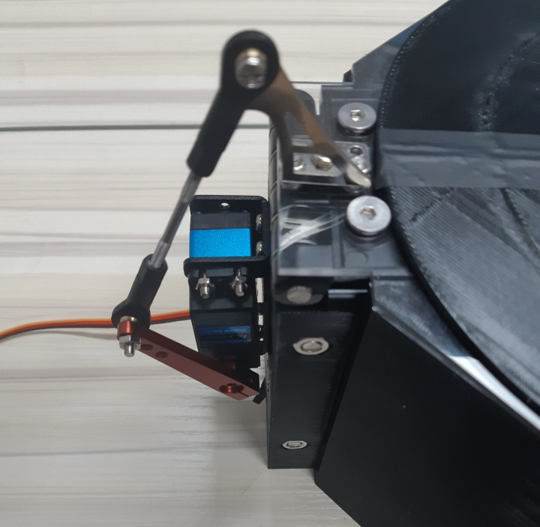
\includegraphics[width = 6cm]{hinge}
	\end{center}
	\caption{개선한 경첩 및 서보모터}
	\label{hinge}
\end{figure}

경통의 후드에서 바흐티노프마스크를 확실하게 제어하기 위해서는 바흐티노프마스크를 적용할 때와 적용하지 않을 때의 구분이 확실해야한다. 이를 확실하게 하기 위해서 바흐티노프마스크를 경첩을 이용하여 큰 각도로 제어하는 방법을 택하였으며, 이를 위해 덮개를 설계할 때 \textrm{Figure} \ref{coverpeice}와 같이 경첩의 높이를 고려하여 제작하였다.

서보모터는 일반적으로 사용하는 DC모터와 다르게 원하는 각도로 모터의 속도를 조절하여 이동시킬 수 있는 모터로,  RC카의 방향제어, 로봇의 관절제어 등의 상황에서 자주 사용되곤 한다. 본 연구에서 사용되는 서보모터는 ‘ds lx3325mg 25kg’ 모델(\textrm{Figure} \ref{motor})으로, 서보모터이지만 360도 회전이 가능한 모델으로, 몸체가 금속으로 되어있어 내구성을 기대할 수 있으며, 축이 톱니모양으로 되어 있기 때문에 제어가 편리하다는 장점을 가지고 있다.

\begin{figure}[h]
	\begin{center}
		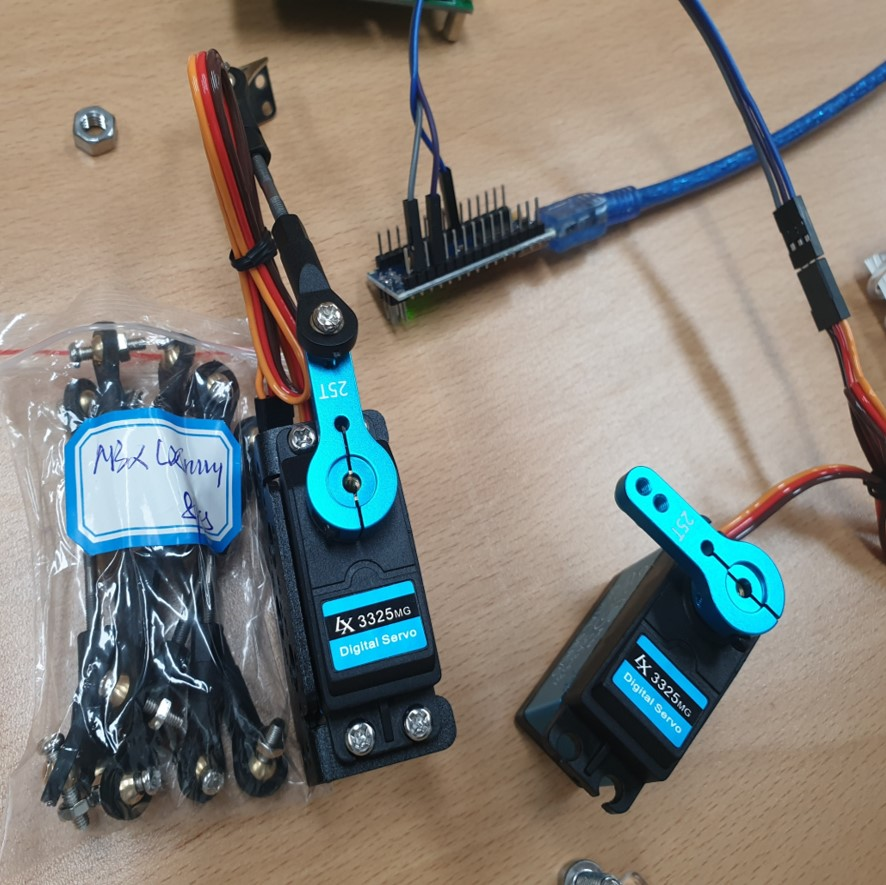
\includegraphics[width = 7cm]{servo1}
	\end{center}
	\caption{사용한 서보모터인 ds lx3325mg 25kg}
	\label{motor}
\end{figure}

\begin{figure}[h]
	\begin{center}
		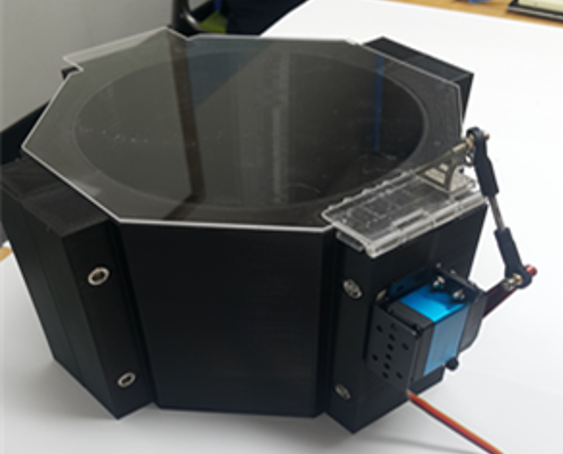
\includegraphics[width = 7.5cm]{servo2}
	\end{center}
	\caption{서보모터를 제작한 후드에 장착한 모습.}
	\label{motorcover}
\end{figure}

서보모터의 경우 구동을 위해 필요한 핀은 3가지이며, 일반적으로 주황색, 빨간색, 갈색의 핀으로 이루어져 있다. 주황색 핀은 모터를 제어할 수 있는 핀이며, 빨간색 핀과 갈색 핀은 각각 $\textrm{5 V}$ 전원과 GND에 연결하여 서보모터를 구동할 수 있다. 서보모터의 경우 \textrm{Figure} \ref{motorcover}처럼 후드의 옆면에 부착시켜 일정한 각도로 제어할 수 있게끔 설계하였다.

서보모터는 후드의 옆면에 부착시켜 제어시킨다. 이 때 정확한 위치에 부착시킬 수 있도록 일정한 간격을 두어 실험을 반복하였으며, \textrm{Figure} \ref{servo}와 같이 적합한 위치를 찾아 고정시켰다. 서보모터로 마스크를 정확하게 제어하기 위해서는 마스크가 완전히 덮개에 고정될 수 있어야 하므로 이에 맞는 각도를 계산하여 사용하여야 한다.

\begin{figure}[ht]
	\begin{center}
		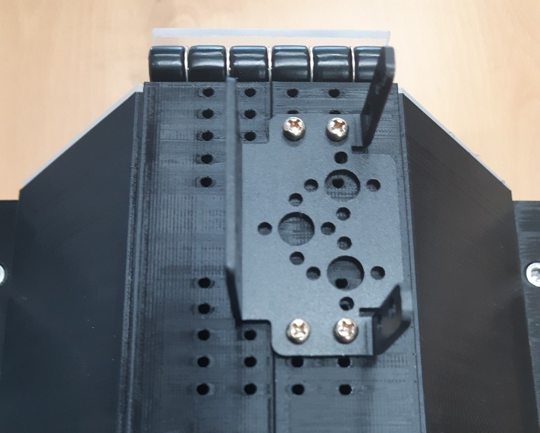
\includegraphics[width = 7cm]{servo3}
	\end{center}
	\caption{후드에 서보모터를 고정하기 위해 볼트를 이용해 고정한 모습}
	\label{servo}
\end{figure}


\subsubsection{바흐티노프마스크 제작}
천체망원경에 사용되는 대부분의 바흐티노프마스크의 도안은 직접 제작이 가능하며, 본 연구의 경우 astrojargon (http://astrojargon.net/MaskGenerator.aspx) 사이트에서 망원경의 사양 및 마스크의 사용 목적에 맞는 적절한 바흐티노프마스크의 도안을 제작하여 사용하였다.

덮개에서 사용되는 방식을 이용한 바흐티노프마스크의 경우 기존처럼 종이나 알루미늄에 프린트된 방식일 경우 덮개에 원하는 모양으로 씌워지지 않을 가능성이 있다. 때문에 주변환경에 영향을 적게 받으면서도 그 면이 평평하여 천체관측을 진행할 때에 영향이 없어야 한다. 

연구 초기에는 아크릴이 이러한 성질을 만족하면서도 쉽게 제작할 수 있으므로 아크릴에 레이저를 쐬여 바흐티노프마스크 모양을 씌우는 방법으로 테스트용 마스크를 제작해보았으나. 이러한 방식을 사용할 경우 \textrm{Figure} \ref{bendmask}처럼 레이저로 인해 열을 받은 아크릴이 변형되어 정밀한 초점 조절이 불가능해지는 경우가 발생하였으며, 아크릴의 두께로 인해 실제로 초점을 조절할 때에 걸리는 여러 가지 변수 또한 무시할 수 없었다.

\bigskip
\begin{figure}[h]
	\begin{center}
		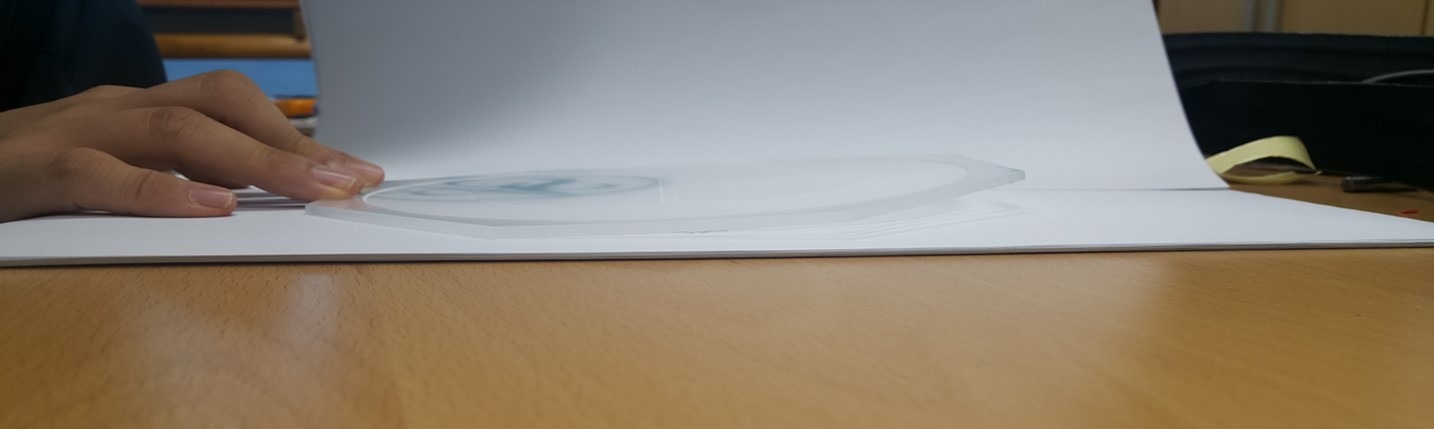
\includegraphics[width = 12 cm]{bendmask}
	\end{center}
	\caption{레이저에 의해 휘어진 아크릴 마스크}
	\label{bendmask}
\end{figure}

때문에 선택한 새로운 방법은 3d프린터를 이용하여 바흐티노프 마스크를 출력하는 것이다. 이 방법으로 얇으면서도 딱딱한 마스크를 사용할 수 있으므로 일반적인 아크릴을 활용한 마스크보다 적은 변수로 바흐티노프 마스크를 덮개에 부착시킬 수 있었다.

Astrojargon을 이용하여 출력한 바흐티노프마스크는 D값을 106, focal length 값을 530으로 출력하였으며, 덮개의 아크릴에 붙이기 편리하도록 지름을 아크릴과 같은 크기로 제작하였다. 출력 과정 중 바흐티노프 사이즈의 크기가 크기 때문에 4조각으로 나누어서 출력하였으며, 빛이 새는 것을 방지하기 위해 나중에 이를 검은 색 테이프로 봉합하였다. 

\begin{figure}[ht]
	\begin{center}
		\begin{tikzpicture}
		\node[anchor=south west,inner sep=0] at (0,0) 
		{
			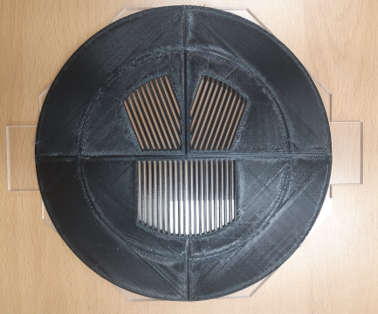
\includegraphics[height=4.5cm]{mask1}
			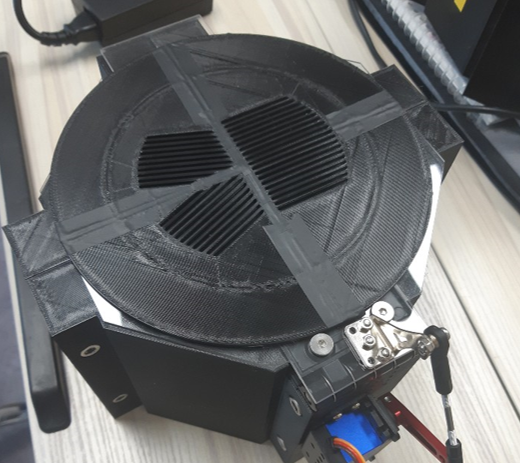
\includegraphics[height=4.5cm]{mask2} 
		};
		\draw (0.3, 4.2) node {(a)};
		\draw (5.9, 4.2) node {(b)};
		\end{tikzpicture}
	\end{center}
	\caption{(a) 4 조각으로 나누어서 출력한 FSQ-106ED 경통의 바흐티노프 마스크 (b) 출력된 마스크를 경통에 붙인 모습. 빛이 새지 않도록 접착부를 검은색 테이프로 접합시켜 고정하였다.}
	\label{mask}
\end{figure}

또한, 3D 프린터의 특성상 한쪽 면은 거친 면, 다른 한쪽 면은 평평한 면을 가지고 있는다. 이 때 거리를 일정하게 하기 위해 평평한 면이 아크릴과 붙는 방향으로 고정시켰다.

\subsubsection{열선 제작}
열선은  니크롬선을 이용하여 제작하였으며, 망원경의 크기와 필요한 열량 등을 고려하여 니크롬선의 저항을 선택한다.

\begin{figure}[h]
	\begin{center}
		\begin{tikzpicture}
		\node[anchor=south west,inner sep=0] at (0,0) 
		{
			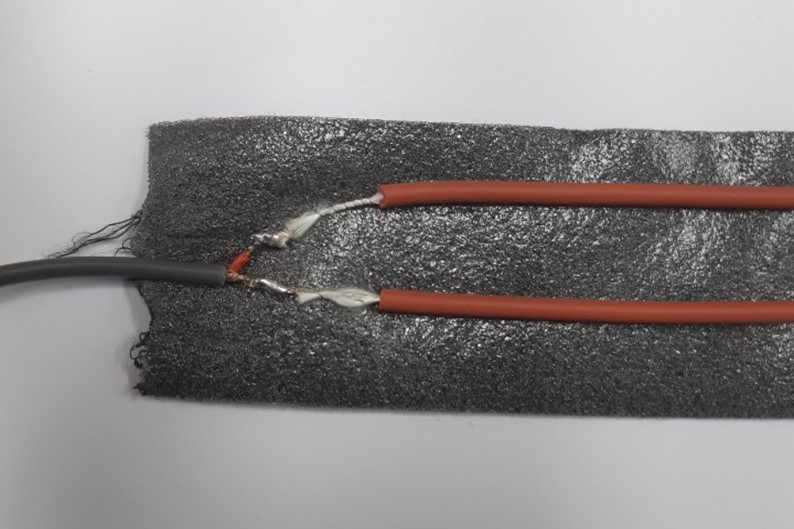
\includegraphics[width=6cm]{thermicline1}
			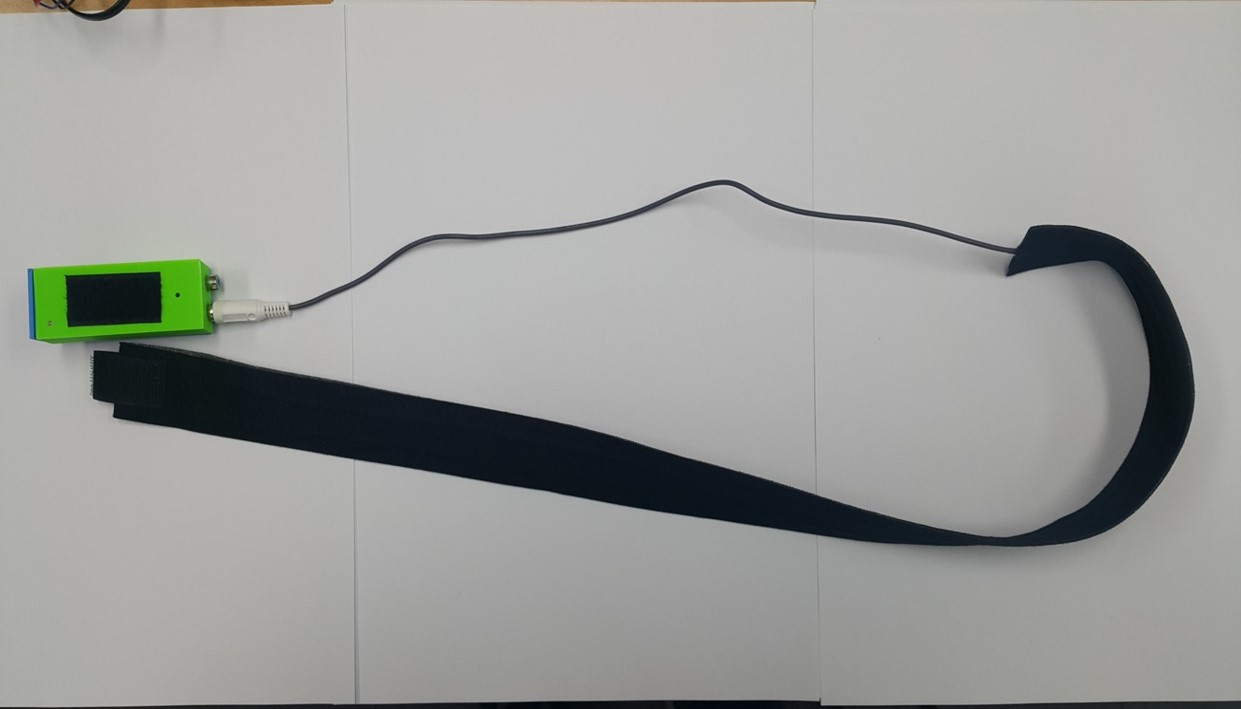
\includegraphics[width=7cm]{thermicline3} 
		};
		\draw (0.3, 3.7) node {(a)};
		\draw (6.4, 3.7) node {(b)};
		\end{tikzpicture}
	\end{center}
	\caption{(a) 제작한 열선의 접합부와 (b) 제작한 열선을 12V에 연결한 모습. 끝에 벨크로가 붙어있어 경통에 둘러 사용할 때 편리하다.}
	\label{thermic}
\end{figure}

열선을 제작하는 방법은 간단하다. 먼저 \textrm{Figure} \ref{thermic}a처럼 끈끈한 면에 히팅케이블을 부착한 뒤에 알맞는 12V어댑터를 분해하여 극을 선과 연결한다. 그리고 열선을 다시 덮어주게 되면 12V 전원을 통해 작동하는 열선을 제작할 수 있다. 열선을 실제로 사용할 시에는 그 편의성을 증대시키기 위해 열선의 끝부분을 벨크로로 연결할 수 있도록 만들게 되며, 이렇게 제작한 열선은 렌즈가 있는 부분을 찾아 둘러주면 벨크로로 끝을 고정시켜 쉽게 망원경에 부착시킬 수 있다.


\subsection{제어부 제작}

\subsubsection{회로 구성}

\textrm{Figure} \ref{circuit01}와

\begin{figure}[h]
	\begin{center}
		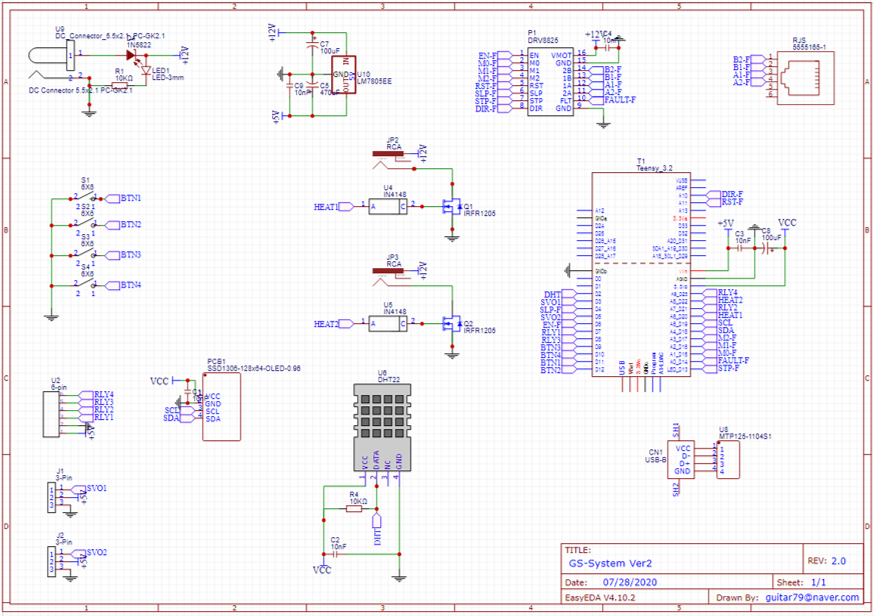
\includegraphics[width = 12cm]{circuit01}
	\end{center}
	\caption{제어부 회로도}
	\label{circuit01}
\end{figure}



\subsubsection{전원 제어}

릴레이 스위치는 전자석으로 이루어진 여러 스위치를 한번에 제어할 수 있도록 제작된 장비이다. 천체관측을 시작 및 종료할 때 가대, CCD, 카메라 등 한번에 여러 가지의 전원을 제어해야 하는데, 릴레이 스위치를 이용하면 한번에 제어할 수 있어 편리하다. 

\begin{figure}[h]
	\begin{center}
		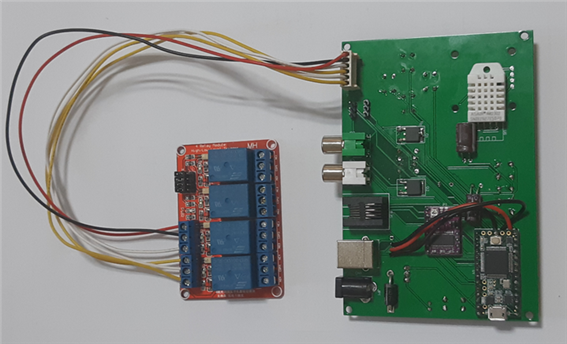
\includegraphics[width = 7.5cm]{relay}
	\end{center}
	\caption{실험에 사용된 릴레이스위치를 모터포커서에 연결시킨 모습}
	\label{relay}
\end{figure}


\textrm{Figure} \ref{relay}와 같이 각각의 스위치를 선으로 연결시켜 mcu의 각 핀에 연결시켜 작동시킬 수 있으며, 함수로 지정하여 이들을 한번에 제어할 수 있도록 하였다.

릴레이 스위치는 6개의 핀으로 이루어져 있으며, 순서대로 $\textrm{+5 V}$, GND, 1, 2, 3, 4의 Relay이다. 때문에 각 핀들을 모두 연결시킨 뒤에 MCU를 이용하여 적절하게 제어할 수 있다. 각각의 기호는 P, Q, R, S이며, 상태만을 나타내기 때문에 서보모터 제어와 마찬가지로 오직 0과 1만을 입력받는다.



\subsubsection{모터 포커서 제어}

이전에 개발된 GS-touch는 바이폴라 스테핑 모터를 제어할 수 있는 모터 포커서로 초점 조절 기능은 이기 때문에 이를 위한 기능들이 주를 이루었다. 때문에 이를 보완하여 덮개를 제어할 수 있도록 추가로 개발할 필요가 있다.


\textrm{Figure} \ref{GStocuh}는 기존에 사용하는 GS-touch의 주요 기능들을 정리한 표이며, GS-touch는 전체적으로 두 가지 부분으로 나눌 수 있다.

\bigskip
\begin{figure}[h]
	\begin{center}
		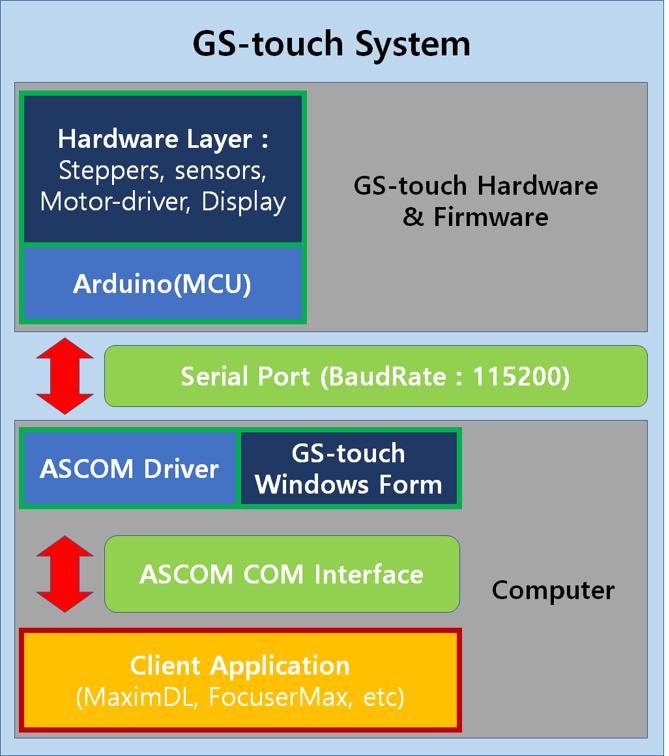
\includegraphics[width = 9.7cm]{GStouch}
	\end{center}
	\caption{GS-touch의 주요 기능}
	\label{GStocuh}
\end{figure}

첫 번째로 GS-touch의 펌웨어는 모터를 직접적으로 제어할 수 있다. DRV8825 모터 드라이버를 활용하여 최대 1/32step의 마이크로 컨트롤을 지원하기 때문에 정밀하게 경통의 길이를 조절할 수 있도록 설계되었으며, 이들을 편하게 관리할 수 있도록 움직인 만큼의 step을 디스플레이에 나타내주며, 이를 원하는 숫자로 초기화하여 얼마나 더 움직였는지 또한 알기 쉽게 하였다. 부가적인 기능으로는 현재 컨트롤러의 위치의 온도와 습도를 알 수 있도록 하여 주변 상황을 쉽게 알 수 있도록 하였다.

두 번째 부분은 GS-touch의 직접적인 제어가 가능하도록 하는 ASCOM 호환 드라이버이다. GS-touch의 드라이버는 ASCOM 홈페이지에서 제공하는 개발자용 버전을 응용하여 C\# 기반으로 제작되었으며, GUI 및 애플리케이션 소프트웨어를 제공하기 때문에 펌웨어에서 제공하는 모든 기능들을 컴퓨터에서 원격으로 사용할 수 있도록 하였다.


비록 GS-touch는 여러 가지 기능을 가지고 있지만 천체망원경의 원격조작에 필요한 여러 기능들을 완벽하게 갖추지는 못하였다. 대표적으로, EEPROM을 사용하지 않았기 때문에 원하는 길이에 step값을 저장할 수 없으며, 온도 및 습도 측정 외의 편의기능 또한 없기 때문에 실제로 사용할 때 많은 불편함이 있다. 본 연구에서는 이러한 단점들을 보완하여 EEPROM을 적용시키고 열선을 사용가능하도록 하는 등의 여러 편의기능들을 개선하였으며, 이를 사용하여 천체망원경용 덮개를 제어할 수 있도록 하였다. 앞으로 실제 천체관측에서의 활용성은 기존에 없었던 천체망원경용 덮개와 더불어 천체망원경의 원격 조작에 큰 도움을 줄 수 있을 것이다.


\subsubsection{서보모터 제어}
바흐티노프마스크를 제어하기 위해서 필요한 조건을 여러 가지가 있겠지만, 가장 중요한 조건 중 하나는 마스크를 사용하는 때와 그렇지 않을 때를 정확히 구분해야하며, 특히 마스크를 사용할 때에는 모든 상황에서 같은 환경을 제공할 수 있어야 한다. 본 연구에서는 경첩을 이용한 각도의 차이로 마스크를 제어하기 때문에 정확한 각도의 이동이 가장 중요하기 때문에 원하는 각도로 정확히 이동할 수 있는 서보모터를 사용하여 정확한 제어가 가능하도록 하였다.

%\subsection{기존 모터포커서 보강}

%앞서 소개했듯이 기존의 모터포커서인 GS-touch는 모터의 초점을 맞추기 위한 기능들에 집중이 되어있기 때문에, 실제로 천체관측 및 원격 천체관측에서는 사용하기 아쉬운 부분들이 많았다. 이에 기존 모터포커서를 보강하였으며, 기존 모터포커서에 비해서 원격 천체관측에 필요한 여러 가지 기능들을 탑재하였다. 본 연구에서 새로 보강한 부분은 다음과 같다.

\subsubsection{열선 제어}
열선또한 정확한 천체관측에 필요한 장비 중 하나이다. 관측을 진행할 때에 경통의 온도가 내려가면 렌즈에 이슬이 맺히게 되는데, 이는 정확한 상을 맺히게 하는데 크게 어려움을 주게 된다. 열선을 경통에 감아놓으면 경통의 온도에 따라서 열선을 제어하여 깨끗한 렌즈를 사용할 수 있게되므로 관측을 편리하게 할 수 있으며, 때문에 천체망원경을 원격제어하기 위해서는 온도를 측정할 수 있는 장비와 열선이 필수적이다. 

열선은 PWM(Puls Width Modulation)을 이용하여 세기를 조절할 수 있다. PWM은 디지털 신호의 밀도로 그 세기를 조절하는 방식으로다 디지털 신호인 0과 1이 출력되는 시간의 비율을 조절하여 원하는 밀도로 제어할 수 있도록 한다. 본 연구에서 직접 제작한 열선을 포함한 대부분의 열선은 12V의 전압을 이용해 제어해야하기 때문에 아두이노의 출력 전원인 5V로는 신호만 제어하고 스위칭 트랜지스터를 이용하여 12V의 전압을 PWM으로 제어할 수 있도록 설계하였다.


앞서 설명하였듯 열선의 제어는 전압의 PWM을 이용하여 실행된다. \textrm{Figure} \ref{PWM}와 같이 시리얼 포트를 통한 입력을 할 때 필요한 기호는 A와 D이며, 0~100의 값을 입력받아 500ms 주기로 값을 변화시킬 수 있도록 설계하였다.

\begin{figure}[ht]
	\begin{center}
		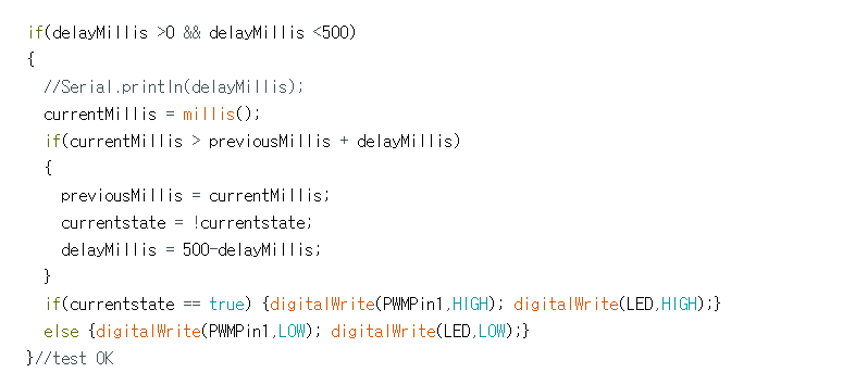
\includegraphics[width = 11cm]{PWMcode}
	\end{center}
	\caption{PWM제어를 위한 코드}
	\label{PWM}
\end{figure}

\subsubsection{EEPROM(Electrically Erasable Read-Only Memory)}

MCU(Micro Controller Unit)내에 원하는 값을 저장하는 방법은 여러 가지가 있다. 일반적으로 펌웨어가 실행되기 전에 변수를 선언하고, loop 문 속에 들어있는 여러 함수들을 통해 그 값을 바꾸는 방법을 사용하곤 한다. 하지만 원격 천체관측을 위한 펌웨어인 만큼, MCU내의 변수만으로 값을 저장하는 것은 상당히 위험하며, 그 전원을 계속 유지할 수 없기 때문에 다른 방법으로 값을 저장할 필요성을 느꼈으며, EEPROM은 기존 방법에 비해 안전하게 값을 저장할 수 있기 때문에 사용하게 되었다.

EEPROM은 대표적인 롬(ROM - read only memory)의 한 종류로서, 전원을 차단해도 저장된 정보를 유지하는 비휘발성 메모리이다. EEPROM은 address를 가지고 있어서 각각의 address 안에 지정된 bytes의 값을 저장할 수 있다. 본 연구에서 사용된 MCU인 Teensy 3.2는 0에서 1023까지의 address지를 가지고 있고 하나의 address에 2048byte, 즉 0부터 255까지의 수를 저장할 수 있다. 모터포커서의 step을 저장하기 위해서는 약 100000범위의 수를 저장할 필요가 있다. GS-touch는 약 -50000에서 50000까지의 수를 저장할 수 있기 때문에 256진법을 활용하여 수를 저장할 수 있도록 설계하였다.

\begin{figure}[h]
	\begin{center}
		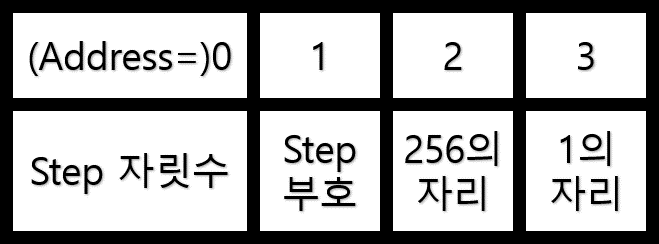
\includegraphics[width = 5 cm]{eeprom1}
	\end{center}
	\caption{EEPROM의 address별 사용 구조. 부호와 값을 절대치를 이용하여 연산하였다.}
	\label{eeprom1}
\end{figure}

\begin{figure}[ht]
	\begin{center}
		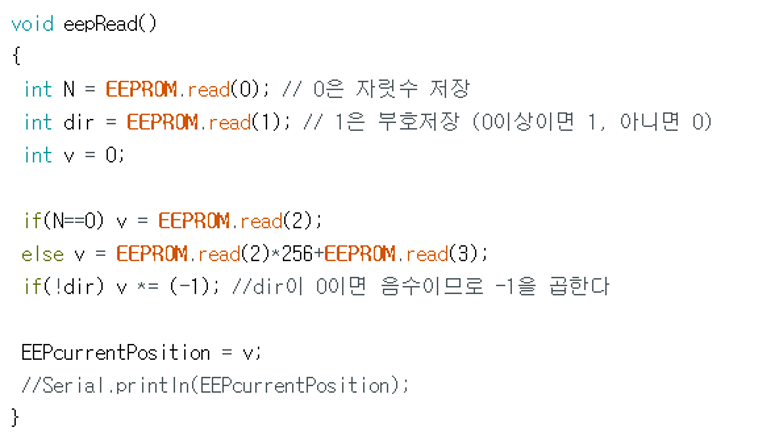
\includegraphics[width = 11cm]{eepread}
	\end{center}
	\caption{EEPROM에서 정보를 읽어오는 과정}
	\label{eepread}
\end{figure}

%https://www.pjrc.com/teensy/td_libs_EEPROM.html

	
	\section{연구 결과}

\subsection{후드 제작}


본 연구에서는 연구 과정에서 제시한 부품들을 3D프린터로 출력 후 조립하여 Fig.\ref{cover}와 같이 이를 천체망원경의 후드처럼 부착시키는 것에 성공하였다. 앞서 소개하였듯, 후드의 지름은 망원경에 따라 달라질 수 있으므로 다른 망원경에 대한 후드를 제작할 때에는 이에 맞추어 새로 제작하여야 한다.
 
\begin{figure}[h]
	\begin{center}
		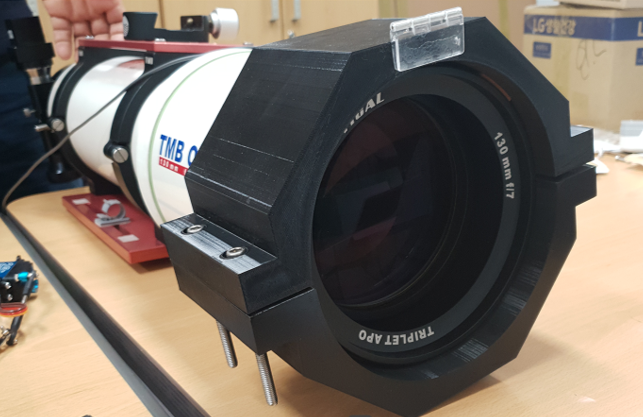
\includegraphics[width = 8cm]{cover}
	\end{center}
\caption{제작한 덮개를 천체망원경에 씌운 모습}
\label{cover}
\end{figure}

경첩은 처음에는 사진에서 사용된 것처럼 플라스틱 소재를 사용하였지만, 이후 금속 소재로 대체하였다. 플라스틱 소재의 경첩은 내구성에서 문제가 있었으며, 3D프린터로 출력한 부품과 접착하기 위해서 여러가지 조건이 필요했기 때문에 안정적이지 않았다. 반면에 금속으로 제작된 경첩은 가운데 뚫려있는 구멍을 활용하여 후드와 안정적으로 결합할 수 있었으며, 내구성또한 뛰어났기 때문에 원격 제어에 적합한 조건들을 갖추고 있다. Fig. \ref{hinge}와 같이 개선된 힌지는 덮개와 아크릴 바흐티노프 마스크 사이를 납작볼트를 이용하여 연결할 수 있으며, 이는 접착제를 이용하여 붙이는 방법보다 간단하고 오래 사용할 수 있다.

 \begin{figure}[h]
	\begin{center}
		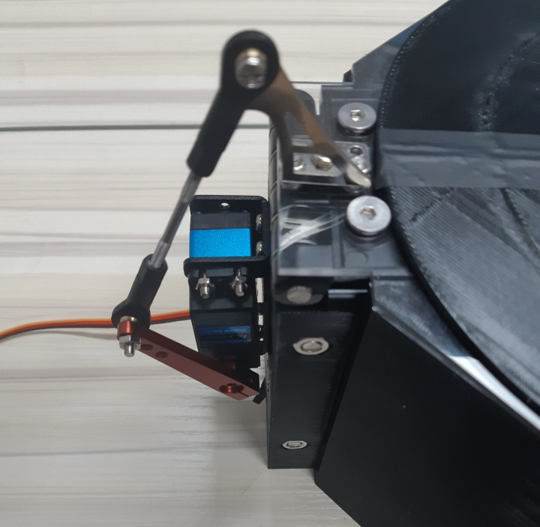
\includegraphics[width = 6cm]{hinge}
	\end{center}
	\caption{개선한 경첩 및 서보모터}
	\label{hinge}
\end{figure}

\subsection{바흐티노프마스크 제작}

Astrojargon을 이용하여 출력한 바흐티노프마스크는 D값을 106, focal length 값을 530으로 출력하였으며, 덮개의 아크릴에 붙이기 편리하도록 지름을 아크릴과 같은 크기로 제작하였다. 출력 과정 중 바흐티노프 사이즈의 크기가 크기 때문에 4조각으로 나누어서 출력하였으며, 빛이 새는 것을 방지하기 위해 나중에 이를 검은 색 테이프로 봉합하였다. 

 
	\begin{figure}[h]
	\begin{center}
		\begin{tikzpicture}
		\node[anchor=south west,inner sep=0] at (0,0) 
		{
			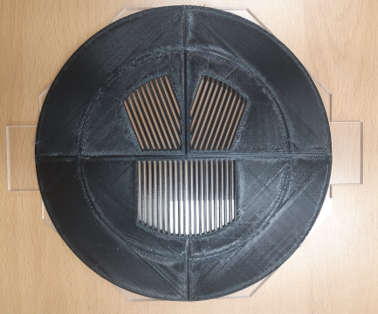
\includegraphics[height=4.5cm]{mask1}
			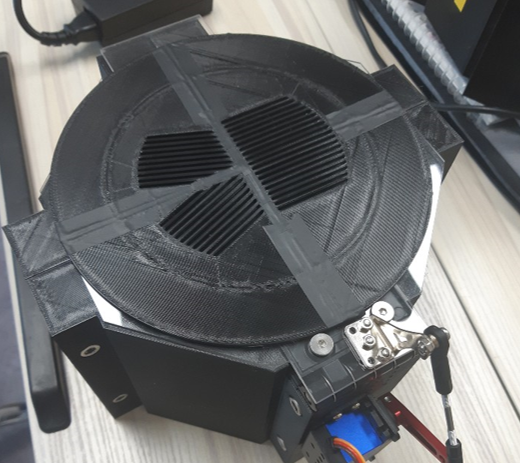
\includegraphics[height=4.5cm]{mask2} 
		};
		\draw (0.3, 4.2) node {(a)};
		\draw (5.9, 4.2) node {(b)};
		\end{tikzpicture}
	\end{center}
	\caption{(a) 4조각으로 나누어서 출력한 FSQ106의 바흐티노프 마스크 (b) 출력된 마스크를 경통에 붙인 모습. 빛이 새지 않도록 접착부를 검은색 테이프로 접합시켜 고정하였다.}
	\label{mask}
	\end{figure}


또한, 3D 프린터의 특성상 한쪽 면은 거친 면, 다른 한쪽 면은 평평한 면을 가지고 있는다. 이 때 거리를 일정하게 하기 위해 평평한 면이 아크릴과 붙는 방향으로 고정시켰다.




\subsection{서보모터 제어}

 서보모터는 후드의 옆면에 부착시켜 제어시킨다. 이 때 정확한 위치에 부착시킬 수 있도록 일정한 간격을 두어 실험을 반복하였으며, Fig. \ref{servo}와 같이 적합한 위치를 찾아 고정시켰다. 

서보모터로 마스크를 정확하게 제어하기 위해서는 마스크가 완전히 덮개에 고정될 수 있어야 하므로 이에 맞는 각도를 계산하여 사용하여야 한다.

\begin{figure}[h]
	\begin{center}
		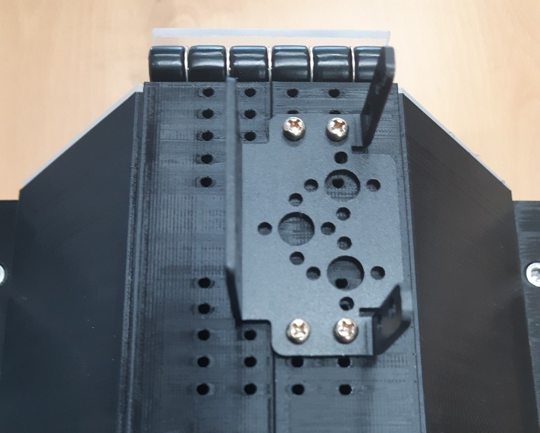
\includegraphics[width = 7cm]{servo3}
	\end{center}
	\caption{후드에 서보모터를 고정하기 위해 볼트를 이용해 고정한 모습}
	\label{servo}
\end{figure}

\subsection{기존 모터포커서 보강}
 제작한 모터포커서는 제어키와 숫자로 이루어져 있는 기호를 통해 통신을 한다. 예를 들어, a에 모터 시계방향 회전을 할당하고 a:100이라는 기호를 입력하면 모터는 시계방향으로 100step만큼 이동하게 되는 것이다. 보강한 모터포커서 또한 이러한 방법을 응용하였으며, 어떤 방법으로 제어에 성공하였는지 서술한다.
 
\subsubsection{열선 제어}

 앞서 설명하였듯 열선의 제어는 전압의 PWM을 이용하여 실행된다. Fig. \ref{PWM}와 같이 시리얼 포트를 통한 입력을 할 때 필요한 기호는 A와 D이며, 0~100의 값을 입력받아 500ms 주기로 값을 변화시킬 수 있도록 설계하였다.
 
  \begin{figure}[h]
 	\begin{center}
 		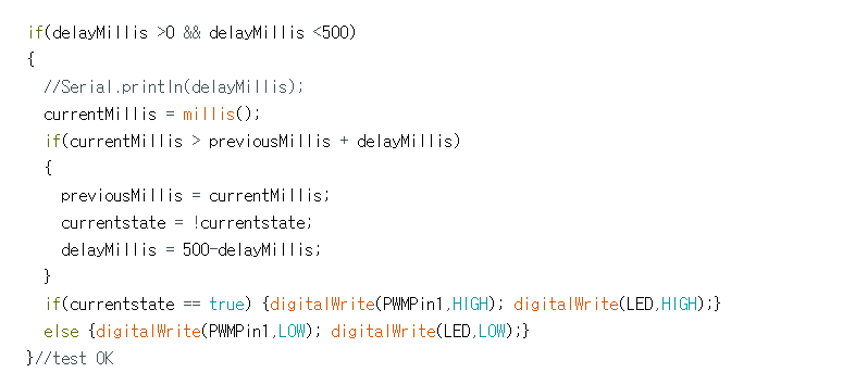
\includegraphics[width = 11cm]{PWMcode}
 	\end{center}
 	\caption{PWM제어를 위한 코드}
 	\label{PWM}
 \end{figure}
 
\subsubsection{EEPROM(Electrically Erasable Read-Only Memory)}

 \begin{figure}[h]
	\begin{center}
		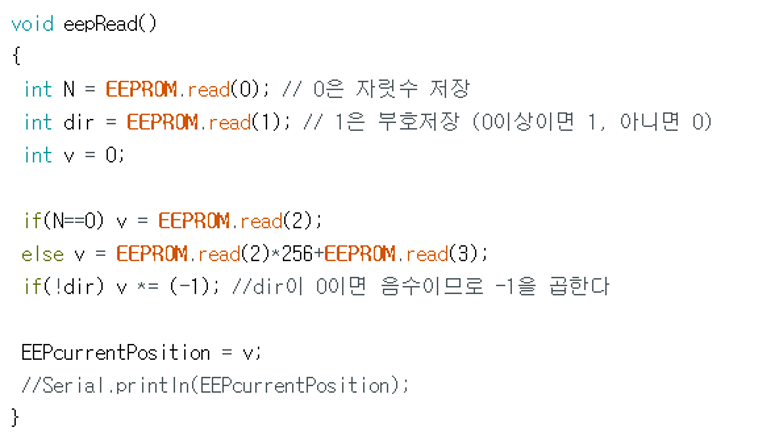
\includegraphics[width = 11cm]{eepread}
	\end{center}
	\caption{EEPROM에서 정보를 읽어오는 과정}
	\label{eepread}
\end{figure}

 모터포커서의 원활한 사용을 위해 저장되어야 하는 값은 모터의 위치를 저장할 수 있는 Position 값이다. Fig.\ref{eepread}은 값을 EEPROM에서 읽어오는 과정을 나타낸 것으로, 모터포커서가 최초로 실행될 때 EEPROM에서 값을 불러오고, 모터를 움직여 값을 변화시킨 직후에 적용된 값을 EEPROM으로 입력시키면 EEPROM값과 모터포커서의 Position 값을 항상 동기화시킬 수 있다.
 
\subsubsection{서보모터 제어}
 일반적인 서보모터 또한 PWM을 응용하여 제어할 수 있으나, 대부분의 라이브러리에서 이미 그 값들을 적용시켜놓은 최적화 함수가 존재한다. 이를 활용하여 서보모터를 원하는 각도로 움직일 수 있도록 펌웨어 상에 코드를 제작하였다. 특히나 OLED를 활용하여 덮개에 부착된 마스크를 정확하게 제어할 수 있도록 하였다.
 
 시리얼 포트를 통한 입력을 할 때 필요한 기호는 N이며, 오직 0과 1만을 입력받아 각각의 상태로 서보모터를 제어한다.

	\begin{figure}[h]
	\begin{center}
		\begin{tikzpicture}
		\node[anchor=south west,inner sep=0] at (0,0) 
		{
			\includegraphics[height=7cm]{mask_status1}
			\includegraphics[height=7cm]{mask_status2} 
		};
		\draw (0.35, 0.3) node {(a)};
		\draw (5.7, 0.3) node {(b)};
		\end{tikzpicture}
	\end{center}
	\caption{(a) 개선된 모터포커서를 이용하여 제어한 덮개 (b) 이 때 개선된 모터포커서에 출력되는 마스크의 상태. 화면 아래의 버튼들을 이용해 상태를 제어할 수 있으며, 제어상태를 확인할 수 있다.}
\label{mask_status}


\end{figure}

\subsubsection{릴레이 스위치}

 릴레이 스위치는 6개의 핀으로 이루어져 있으며, 순서대로 +5v, GND, 1,2,3,4의 Relay이다. 때문에 각 핀들을 모두 연결시킨 뒤에 MCU를 이용하여 적절하게 제어할 수 있다. 각각의 기호는 P, Q, R, S이며, 상태만을 나타내기 때문에 서보모터 제어와 마찬가지로 오직 0과 1만을 입력받는다.
 
 
\newpage
\subsection{개선된 ASCOM 드라이버}


 기존의 모터포커서의 여러 기능들이 추가됨에 따라, 기존에 만들었던 ASCOM 호환 드라이버 또한 업데이트를 할 필요성이 있었다. 때문에 여러가지 기능들을 추가하여 기존의 GUI를 발전시켰으며, Fig\ref{maincontrol}은 발전시킨 ASCOM 드라이버의 GUI의 모습을 나타내었다.
 
 \begin{figure}[h]
	\begin{center}
		\includegraphics[width = 11cm]{maincontrol}
	\end{center}
	\caption{개선된 모터포커서 드라이버의 GUI 모습}
	\label{maincontrol}
\end{figure}

 기존의 모터포커서에서 추가된 기능인 덮개 제어기능, 열선 제어기능, Relay Control을 포함하고 있으며 각각의 Relay가 제어하는 기능들을 적었다.

	\section{결론 및 제언}

\subsection{결론}
	
본 연구를 통하여 천체망원경 모터 포커서 컨트롤러인 GS-touch를 다음과 같이 개발하였다. 

첫째, 아두이노 나노를 기반으로 2상 바이폴라 스테핑 모터 드라이버, OLED 디스플레이어, 온습도 센서 등이 연결된 모터 포커서 컨트롤러인 GS-touch의 하드웨어를 제작하여 구동에 성공하였다. 전원은 DC 12V를 사용하며, 4개의 버튼으로 메뉴를 선택하거나 모터를 정방향 역방향으로 회전시킬 수 있도록 설계하였다.

둘째, GS-touch를 구동할 수 있는 펌웨어을 제작하였다. 펌웨어의 기능은 DRV8825를 이용하여 스테핑 모터를 제어할 수 있도록 하였고, DHT22를 이용하여 온도, 습도 값을 읽어들여 OLED 디스플레이어에 표현할 수 있도록 하였다. 또한 버튼 조작으로 OLED 디스플레이어에 표시되는 메뉴를 조정할 수 있도록 하였다. 

셋째, GS-touch 전용의 ASCOM 드라이버를 개발하여 GS-touch를 PC에 연결하여 ASCOM을 지원하는 MaximDL, FocusMAX 등의 소프트웨어로 구동하는데 성공하였다.

개발된 GS-touch는 기존 제품에 비해 다음과 같은 장점을 가지고 있다. 

첫째, GS-touch는 2상 바이폴라 스텝모터 드라이브인 DRV8825를 사용하여 허용 전류 값이 $3 \textrm{A}$로 micro touch에 비해 월등히 크다. 사진 관측의 경우에는 리듀서, CCD 등 무거운 촬영 장비를 장착하게 되는데 DRV8825의 스펙은 무거운 사진 관측 장비를 장착하고 초점을 조절하는데 무리가 없다. 또한 DRV8825는 1 부터 32 마이크로 스텝까지 펌웨어로 설정 가능하여 포커서의 기어비에 따라 모터 회전 속도를 쉽게 조정할 수 있다. 

둘째, GS-touch는 OLED 디스플레이어를 사용하여 2상 바이폴라 스텝모터 드라이브인 DRV8825본 연구에서 제작된 ASCOM 드라이버의 가장 큰 특징은 직접 개발한 모터제어기를 사용하였기 때문에 그 연동성이 매우 뛰어나다는 것이다. 예를 들어, 모터제어기에 들어있는 마이크로 스텝을 바꾸는 기능은 직접 제작한 ASCOM 드라이버에 그대로 같은 기능을 넣을 수 있었다. 또한 펌웨어에는 없는 기능이더라도 ASCOM 드라이버를 활용하여 더 좋은 활용 방안들을 찾아낼 수 있으며, 

셋째, GS-touch는 DHT22 온습도 센서를 사용하여 온도 뿐 아니라 습도도 파악할 수 있다. 

넷째, GS-touch는 크기가 작아 천체망원경에 장착하기가 용이하다. 

\subsection{제언}

현재 개발된 GS-touch는 초보 단계로서 개선할 수 있는 부분들이 아직 많이 있다. 다음 버전의 하드웨어 부분에서는 버튼 스위치를 좀더 내구성이 좋은 부품으로 교체하는 것이 좋을 것으로 생각된다. 또한 OLED 와 센서의 전원은 아두이노에서 출력되는 전원을 사용하여 외부 전원을 연결하지 않아도 메뉴 조작이 가능하도록 개선할 생각이다.

\begin{description}[font=$\bullet$~\normalfont\scshape\color{red!50!black}]
	\item [Backleash 보정 기능 추가] 모터 포커서를 반대 반향으로 구동할 때 발생할 수 있는 backleash 값을 측정하여 보정할 수 수 있는 기능을 추가할 수 있다.
	\item [MCU 변경] ARDUINO NANO로 펌웨어를 개발할 때 메모리 용량이 작아 어려움을 겪었다. STM32L432KC 같은 는 ARDUINO NANO보다 성능이 좋은 Arduino로, 방향만 반대일 뿐 핀의 순서와 종류가 모두 같아 ARDUINO NANO에 넣었던 펌웨어를 그대로 사용할 수 있다.
	\item [Heating system 추가] 천체 관측시 렌즈에 이슬이 맺혀 관측에 어려움을 겪는 경우가 종종 있다. 이를 해결하기 위하여 날씨가 추운 날에는 모터가 얼어서 돌아가지 않거나 렌즈에 서리가 껴서 초점이 맞아도 맞지 않은 것으로 판단할 수 있다. 따라서 이를 예방하기 위하여 열선을 깔아서 DHT22에서 측정한 온도를 바탕으로 특정한 온도 이하로 내려가게 된다면 열선이 활성화될 수 있게 할 수 있다.
	\item [EEPROM 활용] EEPROM은 Arduino 내부에 저장된 비휘발성 메모리로, 컴퓨터의 ‘RAM’과 같은 역할을 하고 있다. 비휘발성이기 때문에 Arduino를 초기화하거나 껐다가 다시 켰더라도 정보를 저장하고 있다. 
	Arduino별로 한 EEPROM의 주소에 들어갈 수 있는 수의 크기가 달라진다. ARDUINO NANO는 4KB의 EEPROM을 지원하므로 0~255까지의 수를 한 번에 저장할 수 있다. 이렇게 저장할 수 있는 수가 작으므로, 여러 가지 주소를 활용하여 큰 수 또한 나타낼 수 있다.(수를 진법으로 바꾸는 과정과 유사함) 실제로 이를 기반으로 펌웨어를 제작하여 보았지만, 수가 약 32000 이상으로 넘어가는 상황에서는 갑자기 수가 이상하게 커지는 오류가 발견되었고, 이를 고쳐야 할 것이다.
	\item [모터 연결 상태 체크 기능 추가] 모터의 연결 상태는 펌웨어를 실행하는 데 아주 중요하다. 만약 펌웨어가 실행되는 도중에 모터가 연결되지 않으면, 스위치를 움직였을 때 스위치의 숫자는 움직이지만, 모터는 움직이지 않아 결과적으로 숫자의 오류를 불러일으킨다. 또한, 모터를 펌웨어가 실행되는 도중에 연결선을 뽑으면 펌웨어에 에러가 일어나는데, 이 경우 다시 모터를 꽂더라도 정상적으로 실행이 되지 않는다. 따라서 이런 여러 상황에 대하여 모터의 연결 상태를 대비한 에러 코드를 설정해야 숫자와 모터가 오차를 일으키는 일이 없을 것이다.
\end{description}

또한 GS-touch를 활용하여 태양, 행성, 달 등 점 광원이 아닌 천체의 초점 조절 알고리즘을 개발할 생각이다. 앞서 언급한 것처럼 별은 점 광원이므로 FWHM이나 HFD를 이용하여 초점 조절하는 알고리즘이 개발되어 있으나 태양, 행성, 달 등 점 광원이 아닌 천체는 FWHM이나 HDF를 이용한 알고리즘을 적용하기 힘들다. GS-touch를 이용하면 모터 포커서를 정밀하게 제어할 있으므로 태양, 행성, 달 등을 관측할 때 각각의 천체에 적랍한 자동 초점 조절 알고리즘 구현하는데 활용할 수 있을 것으로 생각된다. 
 % Conclusion
	%\clearpage  %%% Appendix를 새 페이지에서 시작
\appendix
\renewcommand{\thesection}{\Alph{section}} %%% TOC에 appendix numbering 재설정
\renewcommand{\thesubsection}{\arabic{subsection}}
\renewcommand{\thesubsubsection}{\arabic{subsubsection}}
\titleformat{\section}[hang] {\normalfont\fontsize{21}{21}\selectfont\bfseries}{\Alph{section}.}{1em}{} %%% Appendix section title의 재설정
\titleformat{\subsection}[hang] {\normalfont\fontsize{16}{16}\selectfont\bfseries}{\Alph{section}.\arabic{subsection}.}{1em}{}
\titleformat{\subsubsection}[hang] {\normalfont\fontsize{14}{14}\selectfont}{\Alph{section}.\arabic{subsection}.\arabic{subsubsection}.}{1em}{}
\titleformat{\paragraph}[hang] {\normalfont\fontsize{12}{12}\selectfont\it}{}{1em}{}
\renewcommand{\theequation}{\thesection.\arabic{equation}} %%% Appendix equation numbering 의 재설정
\renewcommand{\thefigure}{\thesection-\arabic{figure}} %%% Appendix figure numbering 의 재설정
\renewcommand{\thetable}{\thesection-\arabic{table}} %%% Appendix table numbering 의 재설정
\setcounter{equation}{0} %%% Appendix equation starting number의 초기화
\setcounter{figure}{0} %%% Appendix figure starting number의 초기화
\setcounter{table}{0} %%% Appendix table starting number의 초기화
\section{부록}
\begin{table}[h!]
	\begin{center}
		\begin{tabular}{c|c|c|c|c|c|c|c|c}
			\toprule
			&\multicolumn{4}{c|}{Previous Work} & \multicolumn{4}{c}{Our Work}\\
			&\multicolumn{2}{c|}{Blue Lobe} & \multicolumn{2}{c|}{Red Lobe} & \multicolumn{2}{c|}{Blue Lobe} & \multicolumn{2}{c}{Red Lobe}\\
			\textbf{Name} & $\mathbf{v_{out}}$ & $\mathbf{v_{in}}$ & $\mathbf{v_{out}}$ & $\mathbf{v_{in}}$&$\mathbf{v_{out}}$ & $\mathbf{v_{in}}$ & $\mathbf{v_{out}}$ & $\mathbf{v_{in}}$\\
			& [km/s] & [km/s] & [km/s] & [km/s] & [km/s] & [km/s] & [km/s] & [km/s] \\ 
			\midrule
			\multicolumn{9}{c}{Orion A Cloud}\\
			\midrule
			FIR2 & -4.1 & 8.9 & 13.2 & 20.8 &-4.1 & 9.4 & 12.9 & 20.8\\
			FIR3 & -4.1 & 8.9 & 13.2 & 25.1 & -4.1 & 9.25 & 13.0 & 25.1\\
			FIR6b & 1.3 & 8.9 & 13.2 & 21.9 & 1.3 & 9.3 & 12.4 & 21.9\\
			MMS2 & 3.5 & 8.9 & 13.2 & 16.5 & 3.5 & 8.8 & 12.8 & 16.5\\
			MMS5 & 1.3 & 8.9 & 13.2 & 21.9 & 1.3 & 9.5 & 13.1 & 21.9\\
			MMS9 & -4.1 & 8.9 & 13.2 & 26.2 & -4.1 & 9.6 & 13.0 & 26.2\\
			\midrule
			\multicolumn{9}{c}{$\rho$ Ophiuchus Cloud}\\
			\midrule
			Elias 32 & -6.7 & 0.8 & 6.0 & 10.3 & -6.7 & 1.2 & 5.3 & 10.3\\
			IRS 46 & -3.7 & 0.4 & 6.5 & 14.1 & -1.2 & 1.1 & 5.9 & 8.4\\
			VLA 1623 & -3 & 10 & 6.5 & 13 & -3 & 1.2 & 5.3 & 9\\
			BBRCG 24 & N.A. & N.A. & N.A. & N.A. & -5 & 1.2 & 5.7 & 9\\
		\end{tabular}
	\end{center}
	\caption{관측한 원시성들의 적색/청색편이 속도 구간}
\end{table} % Appendix가 없는 경우 주석처리하십시오
	
	\bibliography{bibfile} % 참고문헌
	% BibTeX 코드 쉽게 얻어오는 방법 %
	% Google Scholar 에서 검색한 결과에서 `인용'을 클릭한다.
	% BibTeX 코드를 얻고자 한다면, 하단의 `BibTeX' 을 클릭.
	% 코드가 나온다. Ctrl+A, Ctrl+C로 복사, bibfile에 붙여넣기.
	
	%\begin{summary}
\addcontentsline{toc}{section}{Summary}  %%% TOC에 표시
한글로 졸업논문을 작성한 학생은 반드시 5페이지 내외의 영어 요약문을 작성해야 합니다. 영문으로 작성하는 학생은 이 부분을 작성하지 않아도 됩니다.
\end{summary} % Summary
	%(영어로 작성한 학생은 이 부분을 주석 처리하십시오.)
	%%-----------------------------------------------------
%   감사의 글
%-----------------------------------------------------

%-----------------------------------------------------
%   연구활동 
%-----------------------------------------------------
\begin{researches}
\addcontentsline{toc}{section}{연구활동}  %%% TOC에 표시
\begin{itemize}
\item{2017학년도 교내 R\&E 발표대회에서 우수상 수상}

\end{itemize}
\end{researches} % 감사의 글 & 연구활동
\end{document}